\chapter{Base Detection and Tracking}\label{chap:base_tracking}
One part of the work is focused on the estimation of the state of the moving platform. This is necessary in order to have a good prediction of the final state that the quadrotor must have in order to proper land on the moving car. \\ With the method described in this section, every time we detect the platform we can estimate its position, orientation and velocity vector in world coordinate frame, so we can predict where the platform will be in $t$ seconds and where the quadrotor should go to successfully complete the mission.\\ 


An Extended Kalman Filter  \cite{kalmanfilter} is design in order to have the most reliable value of the state of the platform.\\
Kalman filtering is an algorithm that uses a series of noisy measurements observed over time and produces estimates of unknown variables that tend to be more precise than those based on a single measurement alone, by using Bayesian inference and estimating a joint probability distribution over the variables for each time frame.\\
The algorithm works in a two-step process:
\begin{itemize}
\item In the prediction step, the Kalman filter produces estimates of the current state variables, along with their uncertainties, based on a model of the system:
\begin{align}
\boldsymbol{x}_k = f(\boldsymbol{x}_{k-1},\boldsymbol{u}_k) + \boldsymbol{w}_k
 \label{eq:ekf1}
\end{align}
\item Once the outcome of the next measurement is observed:
\begin{align}
\boldsymbol{z}_k = h(\boldsymbol{x}_{k}) + \boldsymbol{v}_k
 \label{eq:ekf2}
\end{align}
these estimates are updated using a weighted average, with more weight being given to estimates with higher certainty.
\end{itemize}
In the extended Kalman filter, the state transition and observation models don't need to be linear functions of the state but may instead be differentiable functions.\\
($\boldsymbol{w}_k$ and $\boldsymbol{v}_k$ are the process and observation noises which are both assumed to be zero mean multivariate Gaussian noises with covariance $\boldsymbol{Q}_k$ and $\boldsymbol{R}_k$ respectively. $\boldsymbol{u}_k$ is the control vector).

The algorithm is recursive. It can run in real time, using only the present input measurements and the previously calculated state and its uncertainty matrix; no additional past information is required.\\
The Kalman filter does not require any assumption that the errors are Gaussian. However, the filter yields the exact conditional probability estimate in the special case that all errors are Gaussian-distributed.\\
Initialization
\begin{align}
\begin{split}
\boldsymbol{x}_{0|0} = x_0\\
\boldsymbol{P}_{0|0} = P_0
\end{split}
\end{align}
In this case the prediction equations are continuous in time, so for the prediction step of the EKF we have to solve:
\begin{align}
\begin{split}
\boldsymbol{\dot{\hat{x}}}(t) &= f(\boldsymbol{\hat{x}}(t),\boldsymbol{u}(t)) \\
\boldsymbol{\dot{P}}(t) &= \boldsymbol{F}(t) \boldsymbol{P}(t) + \boldsymbol{P}(t)\boldsymbol{F}(t)^{\top } + \boldsymbol{Q}(t)
\end{split}
\end{align}
for $t \in (t_{k-1}, t_k)$ where
\begin{align}
\begin{split}
\boldsymbol{\hat{x}}(t_{k-1}) &= \hat{x}_{k-1|k-1} \\
\boldsymbol{P}(t_{k-1}) &= P_{k-1|k-1}
\\
{\boldsymbol{F}}(t)&=\left.{\frac  {\partial f}{\partial {\boldsymbol{x}}}}\right\vert _{{{\hat  {{\boldsymbol{x}}}}(t),{\boldsymbol{u}}(t)}}  \\
\boldsymbol{\hat{x}}_{k|k-1} &= \boldsymbol{\hat{x}}(t_{k}) \\
\boldsymbol{P}_{k|k-1} &= \boldsymbol{P}(t_{k})
\end{split}
\end{align}
In order to save some computation we can discretize the dynamicin order to have shorter computation during the prediction step of the EKF:
\begin{align}
\begin{split}
\boldsymbol{\hat{x}}_{k|k-1} &= f(\boldsymbol{\hat{x}}_{k-1|k-1},\boldsymbol{u}_k) \\
\boldsymbol{P}_{k|k-1} &= \boldsymbol{F}_{k-1} \boldsymbol{P}_{k-1|k-1}\boldsymbol{F}_{k-1}^{\top } + \boldsymbol{Q}_{k}
\end{split}
\end{align}
where the state transition matrix is defined to be the following Jacobians:
\begin{align}
\begin{split}
\boldsymbol{F}_{k-1}&= \left.{\frac{\partial f}{\partial {\boldsymbol{x}}}} \right \vert_{\hat{\boldsymbol{x}}_{k-1|k-1},\boldsymbol{u}_{k}} 
\end{split}
\end{align}
While the update equations are discrete in time and they yield to the following update step: 
\begin{align}
\begin{split}
\boldsymbol{K}_{k} &= \boldsymbol{P}_{k|k-1} \boldsymbol{H}_{k}^{\top }(\boldsymbol{H}_{k} \boldsymbol{P}_{k|k-1} \boldsymbol{H}_{k}^{\top }+ \boldsymbol{R}_{k})^{-1}
\\
\hat{\boldsymbol{x}}_{k|k} &= \hat{\boldsymbol{x}}_{k|k-1} + \boldsymbol{K}_{k} (\boldsymbol{z}_{k}-h(\hat{\boldsymbol{x}}_{k|k-1}))
\\
\boldsymbol{P}_{k|k} &=(\boldsymbol{I}-\boldsymbol{K}_{k}\boldsymbol{H}_{k})\boldsymbol{P}_{k|k-1}
\end{split}
\end{align}
where the observation matrix is defined to be the following Jacobian:

\begin{align}
\begin{split}
\boldsymbol{H}_{k} = \left.{\frac{\partial h}{\partial {\boldsymbol{x}}}} \right \vert_{\hat{\boldsymbol{x}}_{k|k-1}}
\end{split}
\end{align}

\section{Prediction update: non-holonomic model}
The platform is considered as a car and simulated with a non-holonomic model \ref{fig:nonholonomicmodel}. 
\begin{figure}[!ht]
    \centering
    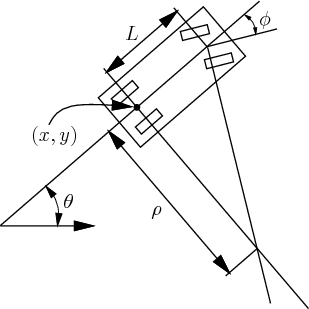
\includegraphics[width=0.5\textwidth]{img/non_holonomic_model.png}
    \caption{Non-holonomic model}
    \label{fig:nonholonomicmodel}
\end{figure}
In this model the state is defined as $\boldsymbol{x} = (x, y, z,\theta , v, \phi)$:
It corresponds to the 3 position in a space $(x,y,z)$ and the yaw angle of the platform $(\theta)$ w.r.t. the world frame, the forward velocity ($v$) and the angle of the front wheels ($\phi$). The system depends on a parameter $L$ that corresponds to the distance between the front and the back wheels.\\
In this model the control input are the change in velocity $v$ and in the angle of curvature $\phi$. \\
The equation of motion in continuous time are:
\begin{align}
\boldsymbol{\dot{x}} = f(\boldsymbol{x},\boldsymbol{u}) \nonumber
\end{align}
\begin{align}
\boldsymbol{\dot{x}} = 
\begin{bmatrix}
\dot{x}  \\[10pt]
\dot{y}  \\[10pt]
\dot{z} \\[10pt]
\dot{\theta} \\[10pt]
\dot{v}  \\[10pt]
\dot{\phi}
\end{bmatrix}
= 
\begin{bmatrix}
v cos(\theta) \\[10pt]
v sin(\theta) \\[10pt]
 0 \\[10pt]
\frac{v}{L}tan(\phi)\\[10pt]
u_1 \\[10pt]
 u_2 
\end{bmatrix}
\label{eq:ekfcomponents}
\end{align}
It is possible to discretize these dynamics in $t \in (t_{k-1}, t_k)$ with a first order finite difference:
\begin{align}
\boldsymbol{\dot{x}} \approx \frac{\boldsymbol{x}_k - \boldsymbol{x}_{k-1} }{dt} \approx f(\boldsymbol{x}_{k-1},\boldsymbol{u}_k) \nonumber
\end{align}
with $\boldsymbol{x}_k = \boldsymbol{x}(t_k)$, $\boldsymbol{x}_{k-1} = \boldsymbol{x}(t_{k-1})$, $dt = t_k - t_{k-1}$
\begin{align}
\boldsymbol{x_k} = 
\begin{bmatrix}
x_k  \\[10pt]
y_k  \\[10pt]
z_k \\[10pt]
\theta_k \\[10pt]
v_k  \\[10pt]
\phi_k
\end{bmatrix}
= 
\begin{bmatrix}
 x_{k-1} + dt \big(v_{k-1} cos(\theta_{k-1})\big) \\[10pt]
 y_{k-1} + dt \big(v_{k-1} sin(\theta_{k-1})\big) \\[10pt]
 z_{k-1} \\[10pt]
 \theta_{k-1} + dt\Big(\frac{v_{k-1}}{L}tan(\phi_{k-1}) \Big)\\[10pt]
v_{k-1} + dt \big(u_{1k}\big) \\[10pt]
\phi_{k-1} + dt \big(u_{2k}\big) 
\end{bmatrix}
\label{eq:realstate}
\end{align}

In order to solve the former system, we have anyway to find a numerical solution. For this purpose we use a    
Runge-Kutta scheme  \cite{wiki_runge_kutta}.\\
In numerical analysis, the Runge-Kutta methods are a family of implicit and explicit iterative methods used in temporal discretization for the approximate solutions of ordinary differential equations.\\
The most widely known member of the Runge-Kutta family is generally referred to as RK4.\\
Let an initial value problem be specified as follows:
\begin{align}
\begin{split}
{\dot {y}}&=f(t,y) \\
y(t_{0})&=y_{0}
\end{split}
\end{align}
$y$ is an unknown function (scalar or vector) of time $t$, which we would like to approximate and the function $f$ and the data $t_{0}$, $y_{0}$ are given.\\
Now pick a step-size $h > 0$ and define
\begin{align}
\begin{split}
y_{k+1}&=y_{k}+{\tfrac {h}{6}}\left(\alpha_{1}+2\alpha_{2}+2\alpha_{3}+\alpha_{4}\right),\\
t_{k+1}&=t_{k}+h
\end{split}
\end{align}
for $k = 0, 1, 2, 3, ...,$ using
\begin{align}
\begin{split}
\alpha_{1}&=f(t_{k},y_{k}),\\
\alpha_{2}&=f(t_{k}+{\frac {h}{2}},y_{k}+{\frac {h}{2}}\alpha_{1}),\\
\alpha_{3}&=f(t_{k}+{\frac {h}{2}},y_{k}+{\frac {h}{2}}\alpha_{2}),\\
\alpha_{4}&=f(t_{k}+h,y_{k}+h\alpha_{3}).
\end{split}
\end{align}
Here  $y_{k+1}$ is the RK4 approximation of $y(t_{k+1})$, and it is determined by the present value ($y_{k}$) plus the weighted average of four increments.

\subsubsection{Straight and circular path}
We assume the input $u_1$ and $u_2$  are equal to zero. In this way we can have three type of movement:
\begin{itemize}
\item the platform can be static ($v_f(0) = 0$)
\item it can move in a straight line ($v_f(0) \neq 0$ and $\phi(0) = 0$)
\item it can move in a circle ($v_f(0) \neq 0$ and $\phi(0) \neq 0$)
\end{itemize}
As described in charapter \label{chap:thechallenge}, the final trajectory of the platform is only a composition of a linear and a circular movement (for a given determinate amount of time). So this model can be used also in the final implementation.

\section{Measurement update}
From equation \ref{eq:ekfcomponents} we have the variables that describe the state of the moving car. We have to be able to measure some of these components in order to have the second step of our EKF. \\
What we are using is a camera with which we are able to identify the moving platform and estimate the relative position and orientation. At this point knowing the position of the camera in the real world we can measure the following vector $\boldsymbol{z} = (x, y, z,\theta)$. It corresponds to the 3 position in a space $(x,y,z)$ and the yaw angle of the platform $\theta$ w.r.t. the world frame.
The measurement equations are simply:
\begin{align}
\boldsymbol{z_k} = 
\begin{bmatrix}
x_k  \\[10pt]
y_k  \\[10pt]
z_k \\[10pt]
\theta_k
\end{bmatrix}
\label{eq:realmeasure}
\end{align}

In the different phases we have to use different methods measure  $\boldsymbol{z}$ detecting and tracking the base:
\begin{itemize}
\item to be able to find the platform in the minimum amount of time, at the beginning, we need to inspect the area from a very high altitude. From this height we can see just a few features of the moving car and then the pose estimation are noisy. Furthermore we do not have any assumption on the initial condition of the platform, we just know the magnitude of constant forward velocity $|v_{tan}|$, so we do not know before if at a certain time $t$ the car is moving in a straight line or in a curve, we have to estimate it, and this is possible only tracking the platform for several seconds. 
\item after knowing the type of movement and a rough pose estimation of the moving car, we can use these information to improve our state estimation: getting close to the platform without loosing the tracking, starting a more precise measure (base on tag detection), and filtering the measurements with a theoretical model of the movement.
\end{itemize}
\subsection{From high altitude}
To find the car we assume that the platform is the only white square moving on the arena.
Base on this assumption, we analyze the images from the down looking camera to find a moving white square and calculate its optical flow to predict its future position.

We perform the following passages:
\begin{itemize}
\item threshold the image in order to find the white features.
\item find all the close shapes in the image.
\item select only the shapes with
\begin{itemize}
\item 4 edges
\item convex contour
\item angles between edges close to $\frac{\pi}{2}$
\end{itemize}
\end{itemize}
At this point we have the position of the four corners of all the squares in the image.\\
Now we try to calculate the optical flow of these points through the sequence of images and we track only the points that are moving with a velocity comparable to the one known $v_{tan}$.\\

The optical flow methods \cite{beauchemin1995computation} try to calculate the motion, for each pixel, between two image frames which are taken at times $t$ and $t+\Delta t$. \\
For a 2D dimensional case a pixel at location $(x,y,t)$ with intensity $I(x,y,t)$ will have moved by $\Delta x$,$\Delta y$ and $\Delta t$ between the two image frames. \\
To solve this problem, the core assumption is the brightness constancy constraint:
\begin{align}
I(x,y,t) = I(x+\Delta x, y + \Delta y, t + \Delta t)
\end{align}
Assuming the movement to be small, the image constraint at $I(x,y,t)$ with Taylor series can be developed to get:
\begin{align}
I(x+\Delta x,y+\Delta y,t+\Delta t) = I(x,y,t) + \frac{\partial I}{\partial x}\Delta x+\frac{\partial I}{\partial y}\Delta y+\frac{\partial I}{\partial t}\Delta t.
\end{align}
From these equations it follows that:
\begin{align}
 \frac{\partial I}{\partial x}\frac{\Delta x}{\Delta t}+\frac{\partial I}{\partial y}\frac{\Delta y}{\Delta t}+\frac{\partial I}{\partial t}\frac{\Delta t}{\Delta t} = 0
\end{align}
which results in
\begin{align}
 I_{x}V_x+I_{y}V_y+I_{t}= 0
\end{align}
where $V_x,V_y$ are the $x$ and $y$ components of the velocity or optical flow of $I(x,y,t)$ and $I_{x}$, $I_{y}$, $I_{t}$ are the derivatives of the image at $(x,y,t)$ in the corresponding directions.\\
Thus:
\begin{align}
 \nabla I^T\cdot\vec{V} = -I_t
\end{align}
This is an equation in two unknowns and cannot be solved as such. This is known as the aperture problem of the optical flow algorithms. To find the optical flow another set of equations is needed, given by some additional constraint. All optical flow methods introduce additional conditions for estimating the actual flow.\\
In our implementation we use the Lucas-Kanade method \cite{lucas1981iterative}.
This method assumes that the displacement of the image contents between two nearby frames is small and approximately constant within a neighborhood of the point p under consideration. Thus the optical flow equation can be assumed to hold for all pixels within a window centered at $p$. Namely, the local image flow vector $(V_{x},V_{y})$ must satisfy:

\begin{align}
\begin{split}
I_{x}(q_{1})V_{x}+I_{y}(q_{1})V_{y}=-I_{t}(q_{1})  \\
I_{x}(q_{2})V_{x}+I_{y}(q_{2})V_{y}=-I_{t}(q_{2})  \\
\vdots \\
I_{x}(q_{n})V_{x}+I_{y}(q_{n})V_{y}=-I_{t}(q_{n}) 
\end{split}
\end{align}

Where $q_{1},q_{2},\dots ,q_{n}$ are the pixels inside the window, and $I_{x}(q_{i}),I_{y}(q_{i}),I_{t}(q_{i})$ are the partial derivatives of the image $I$ I with respect to position x, y and time t, evaluated at the point $q_{i}$ and at the current time.\\
These equations can be written in matrix form $Av=b$, where
\begin{align}
A={\begin{bmatrix}I_{x}(q_{1})&I_{y}(q_{1})\\[10pt]I_{x}(q_{2})&I_{y}(q_{2})\\[10pt]\vdots &\vdots \\[10pt]I_{x}(q_{n})&I_{y}(q_{n})\end{bmatrix}},\quad \quad v={\begin{bmatrix}V_{x}\\[10pt]V_{y}\end{bmatrix}},\quad {\mbox{and}}\quad b={\begin{bmatrix}-I_{t}(q_{1})\\[10pt]-I_{t}(q_{2})\\[10pt]\vdots \\[10pt]-I_{t}(q_{n})\end{bmatrix}}
\end{align}

This system has more equations than unknowns and thus it is usually over-determined. The Lucas-Kanade method obtains a compromise solution by the least squares principle. Namely, it solves the $2\times2$ system:
\begin{align}
\begin{split}
A^{T}Av=A^{T}b\\
{\mathrm  {v}}=(A^{T}A)^{{-1}}A^{T}b
\end{split}
\end{align}
\begin{align}
{\begin{bmatrix}V_{x}\\[10pt]V_{y}\end{bmatrix}}={\begin{bmatrix}\sum _{i}I_{x}(q_{i})^{2}&\sum _{i}I_{x}(q_{i})I_{y}(q_{i})\\[10pt]\sum _{i}I_{y}(q_{i})I_{x}(q_{i})&\sum _{i}I_{y}(q_{i})^{2}\end{bmatrix}}^{{-1}}{\begin{bmatrix}-\sum _{i}I_{x}(q_{i})I_{t}(q_{i})\\[10pt]-\sum _{i}I_{y}(q_{i})I_{t}(q_{i})\end{bmatrix}}
\end{align}
With this method we can track the interesting points from frame to frame, calculate direction and velocity of the car and so predict where it will be after a time $t$.\\
\begin{figure}[!htbp]
  \centering
  {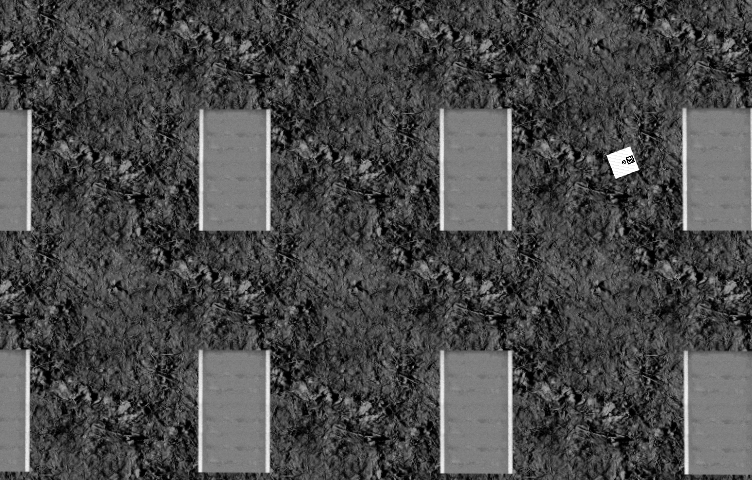
\includegraphics[width=0.45\textwidth]{img/18730previousImage.png}\label{fig:original}}
  \hfill
  {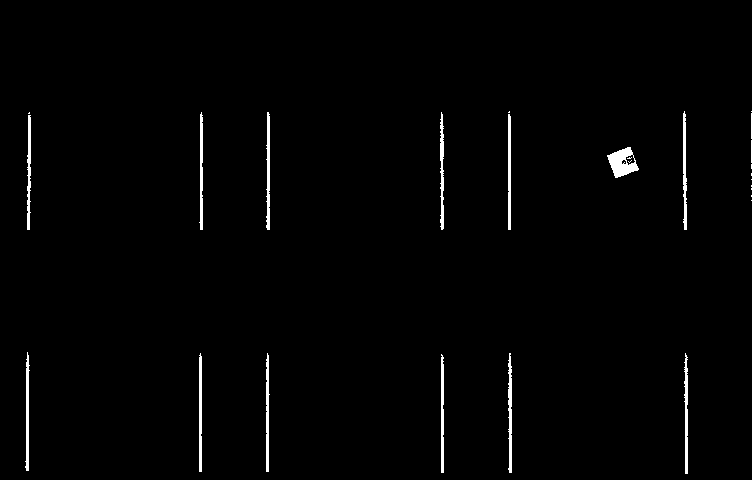
\includegraphics[width=0.45\textwidth]{img/18730_thresholded.png}\label{fig:threshold}}
  \vspace{1cm}
  
  {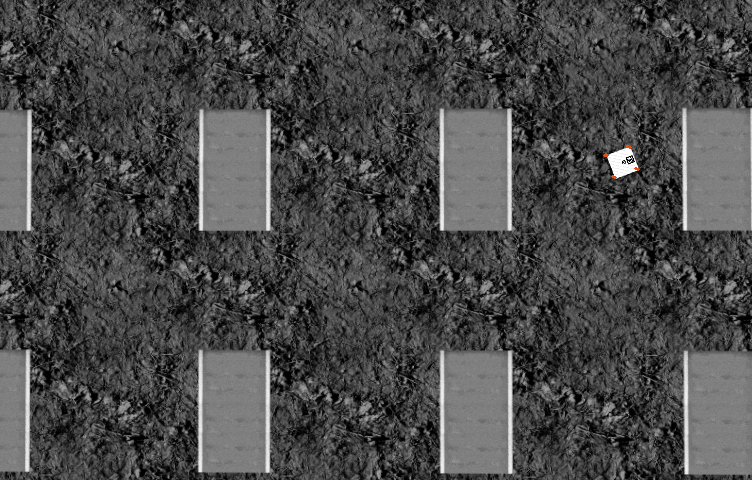
\includegraphics[width=0.45\textwidth]{img/18741_optical_flow.png}\label{fig:optical1}}
  \hfill
  {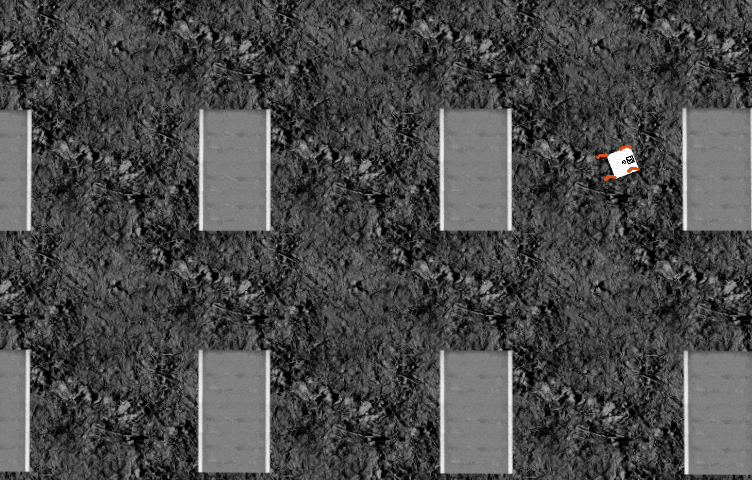
\includegraphics[width=0.45\textwidth]{img/18758_optical_flow.png}\label{fig:optical2}}
  \vspace{1cm}
  
  {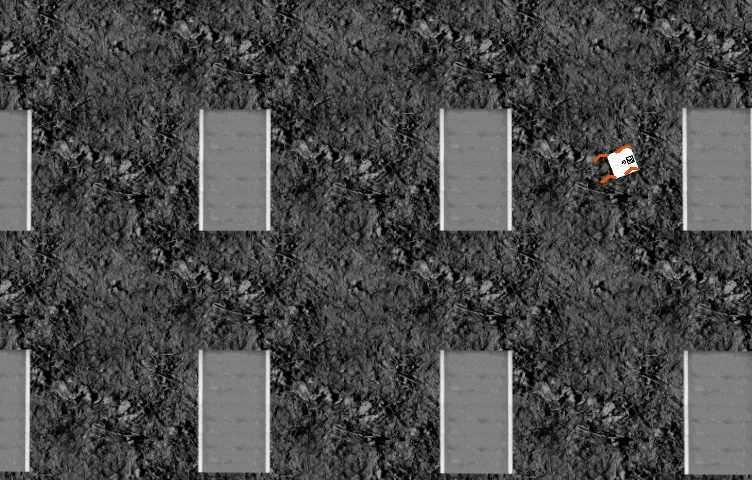
\includegraphics[width=0.45\textwidth]{img/18777_optical_flow.png}\label{fig:optical3}}
  \hfill
  {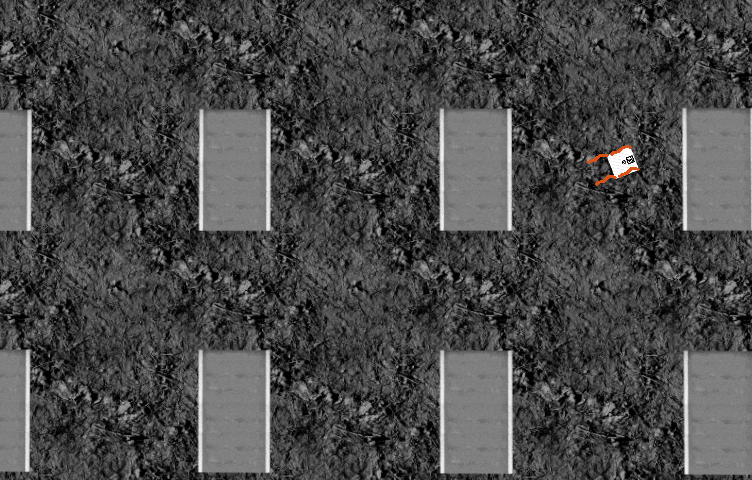
\includegraphics[width=0.45\textwidth]{img/18800_optical_flow.png}\label{fig:optical4}}
   
  \vspace{1cm}
  {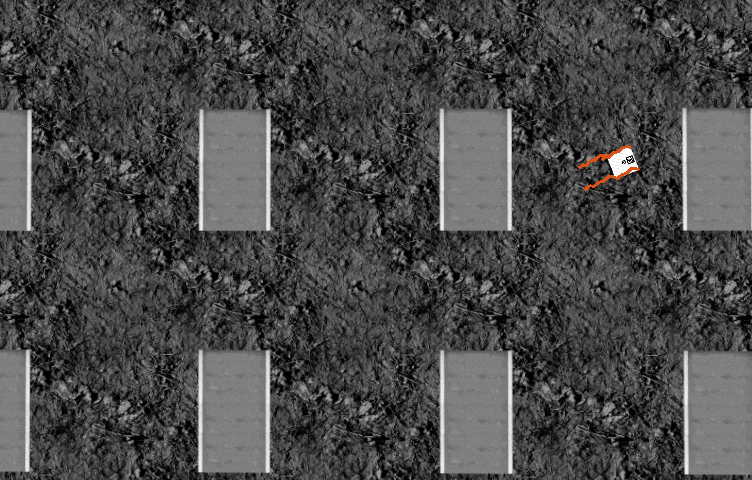
\includegraphics[width=0.45\textwidth]{img/18856_optical_flow.png}\label{fig:optical5}}
  \hfill
  {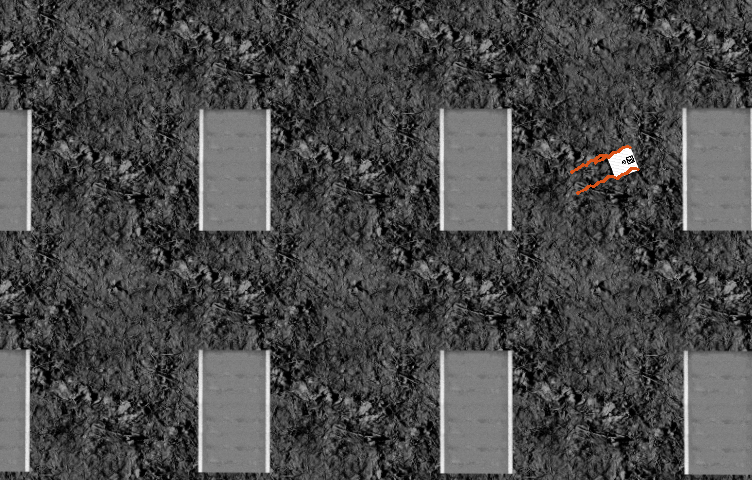
\includegraphics[width=0.45\textwidth]{img/18881_optical_flow.png}\label{fig:optical6}}
 
  \caption{A sequence of images where the moving car is detected and tracked. First image is the original image. Then the one after thresholding. Then all the subsequent images where the corners of the platform are tracked.}
  \label{fig:optical_folw_sequence}
\end{figure} 

\subsubsection{From images to real world}
After tracking the platform in the images, we have to find its position in the 3D real world. This position is calculate using the pinhole model of the camera \cite{weng1992camera}:
\begin{align}
wm = A [R|t]M
 \label{eq:pinholemodel}
\end{align}
In expanded form:
\begin{align}
{w\begin{bmatrix}
u \\[10pt]
v  \\[10pt]
1
\end{bmatrix}}=
{\begin{bmatrix}\
f_x & 0 & c_x \\[10pt]
0 & f_y &c_y \\[10pt]
0 & 0 & 1
\end{bmatrix}}
{\begin{bmatrix}\
r_{11} & r_{12} & r_{13} & t_{x} \\[10pt]
r_{21} & r_{22} & r_{23} & t_{y} \\[10pt]
r_{31} & r_{32} & r_{33} & t_{z}
\end{bmatrix}}
{\begin{bmatrix}
X \\[10pt]
Y \\[10pt]
Z \\[10pt]
1
\end{bmatrix}}
\end{align}
Where:
\begin{itemize}
 \item $m$ homogeneous coordinate of the projection point in pixel.
  \item $M$ homogeneous coordinate of a 3D point in the world coordinate frame.
 \item $A$ is the camera matrix or the matrix of intrinsic parameters. It is Composed by $f_x,f_y$ the focal lengths and $c_x,c_y$ the principal point.
 \item $[R|t]$ is the joint rotation-translation matrix or matrix of extrinsic parameters. It express the camera motion around the static scene. This matrix denote the coordinate system transformations from 3D world coordinates to 3D camera coordinates. The position $C$ of the camera expressed in world coordinates is $C=-R^{{-1}}t=-R^{T}t$.
\end{itemize}

We can calculate the depth of the platform using the known dimension of the base: given the length $l_w$ of the square in the real world and the average dimension of the edges in the image $l_i$, we can calculate the depth with respect to the camera frame 
\begin{align}
z = \frac{l_w f}{l_i}
\end{align}
To calculate the dimension $l_i$ we need at least 3 corner of the base and we calculate all the pairwise distances between the corners \ref{fig:platform_profile}:
\begin{itemize}
\item if we have 4 corners there are 6 different distances: 4 of which equal to $l_i$ and 2 $\sqrt{2}l_i$
\item if we have 3 corners there are 3 different distances: 2 of which equal to $l_i$ and 1 $\sqrt{2}l_i$
\end{itemize}
This approximation is not really precise when we see the platform with a camera not perpendicular to the base, but we need just a rough approximation of the height in this first phase.
\begin{figure}[!htbp]
  \centering
  {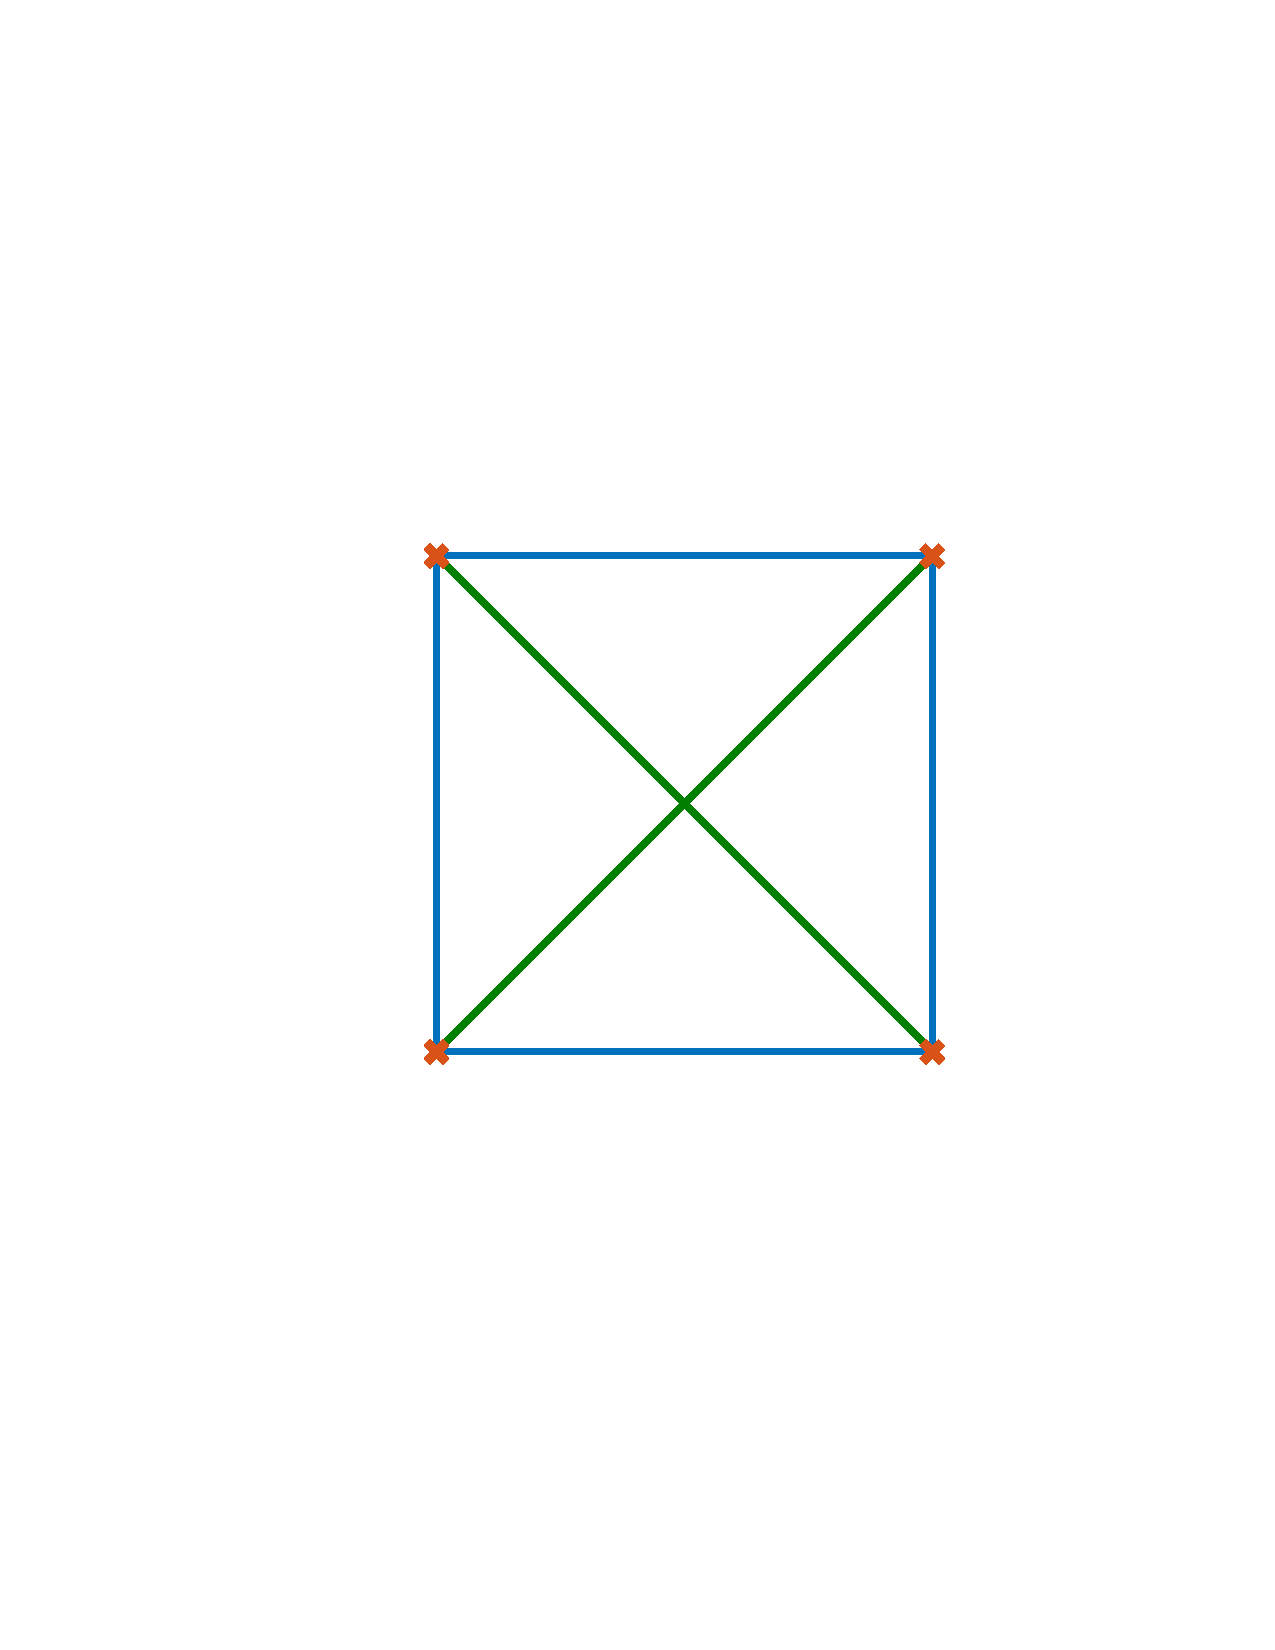
\includegraphics[width=0.3\textwidth]{img/platform_4_edges.pdf}\label{fig:4_corners}}
  \hspace{5em}
  {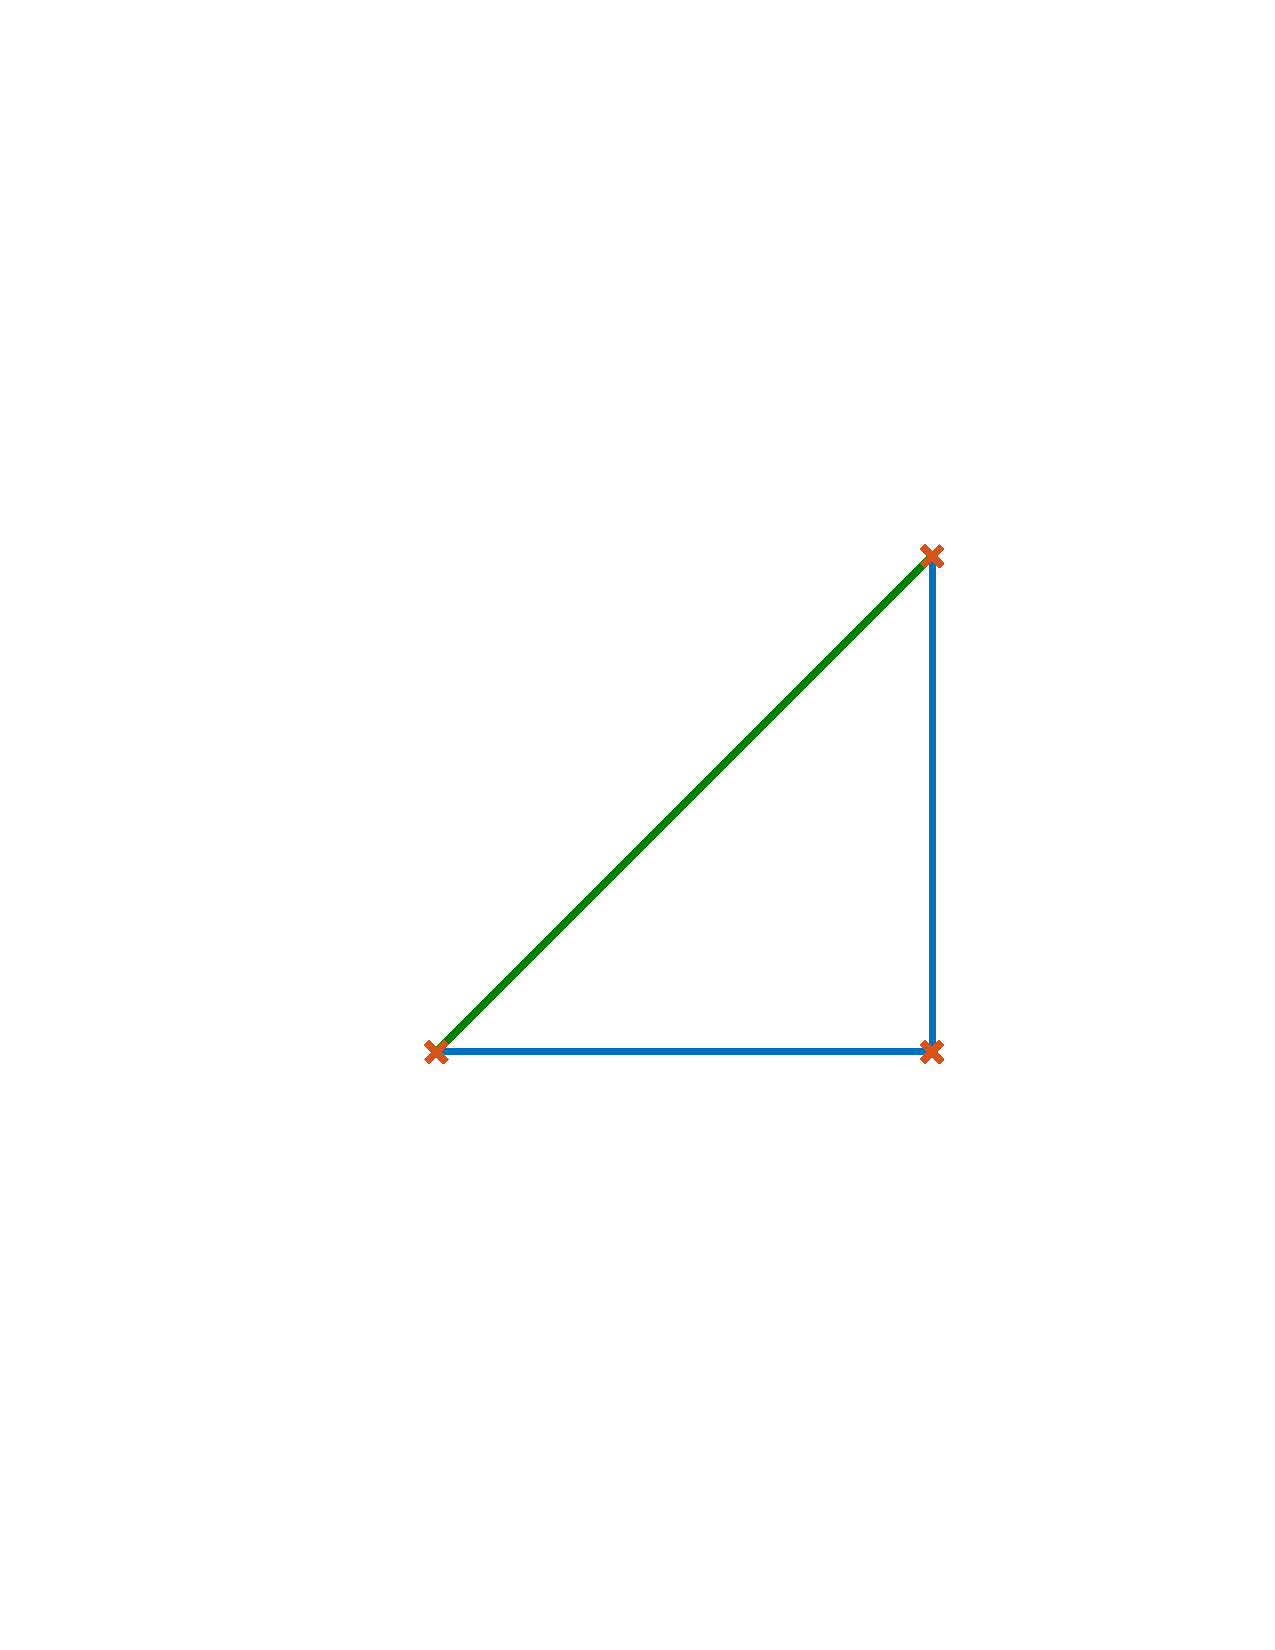
\includegraphics[width=0.3\textwidth]{img/platform_3_edges.pdf}\label{fig:3_corners}}
  \caption{Model of the square platform detected on the image. Red crosses corner detected. Blue lines edges with length $l_i$. Green lines edges with length $\sqrt{2}l_i$ }
  \label{fig:platform_profile}
\end{figure} 

If this depth $z!=0$ we can  solve the system of equation \ref{eq:pinholemodel} finding an unique solution using the following equivalent equations:
\begin{align}
\begin{split}
x &= z\frac{u-c_x}{f_x}\\[10pt]
y &= z\frac{v-c_y}{f_y}\\[10pt]
{\begin{bmatrix}
x \\[10pt]
y \\[10pt]
z
\end{bmatrix}} &= 
R {\begin{bmatrix}
X \\[10pt]
Y \\[10pt]
Z
\end{bmatrix}} + t
\end{split}
\end{align}

A better method to find the position of the platform, without the approximation of the depth $z$ is to resolve a Perspective-n-Point problem  \cite{quan1999linear}
that estimates the pose of a camera given a set of n 3D points in the world and their corresponding 2D projections in the image. The only issue is that to solve this problem without ambiguity the minimum number of points is 4, and sometimes we can track only 3 corners of the base, but when all the 4 points are available we solve the correspondent PnP problem to find a better estimation of the base position.\\

\subsection{From low altitude}
When the quadrotor is closer to the landing platform more features can be seen from the camera. This allow to design a base that helps the measure of the pose of the moving car.\\
In the final challenge \label{chap:thechallenge} the platform will be as depicted in figure \ref{fig:finalplatform}, while for the first testing another design is considered \ref{fig:tempplatform}, in order to use preexisting algorithm that allow pose estimation with respect to the camera. The platform we are using is decorated with Augmented-Reality Tags. AR Tags are planar markers used to easily make virtual objects and animations appear to enter the real world. They also allows video tracking capabilities that calculate the real camera position and orientation relative to square physical markers in real time. \\
To reduce the sensitivity to lightning conditions and camera settings planar marker systems typically use bitonal markers (black and white), so there is no need to identify shades of gray, and the decision made per pixel is reduced to a threshold decision. The markers consist of a square black border and a pattern in the interior to an unique identification, when more the one marker is used in the application.\\
There are several methods to detect and calculate the pose of the markers. Some methods (as ARToolKit \cite{kato1999marker}), use a fixed global threshold to detect squares, but these methods are very sensitive to varying lighting conditions. On the other hand, other algorithms (as ARTag \cite{fiala2010designing}), use an edge based approach, so one need not to deal with thresholds under different illumination conditions and the algorithm can cope with broken sides and missing corners to a certain extent. 
Both algorithms find on the image the contour of the marker, the four corners of every potential marker are used to calculate a homography in order to remove the perspective distortion. This perspective undistortion is done solving a Perspective-n-Point problem \cite{quan1999linear}.\\
Once the internal pattern of a marker is brought to a canonical front view one can sample a grid of $N \times N$ (typically $5 \times 5$ or $6 \times 6$) points in order to understand the code related to the tag identified, and the orientation of the tag.

\begin{figure}[!htbp]
    \centering
    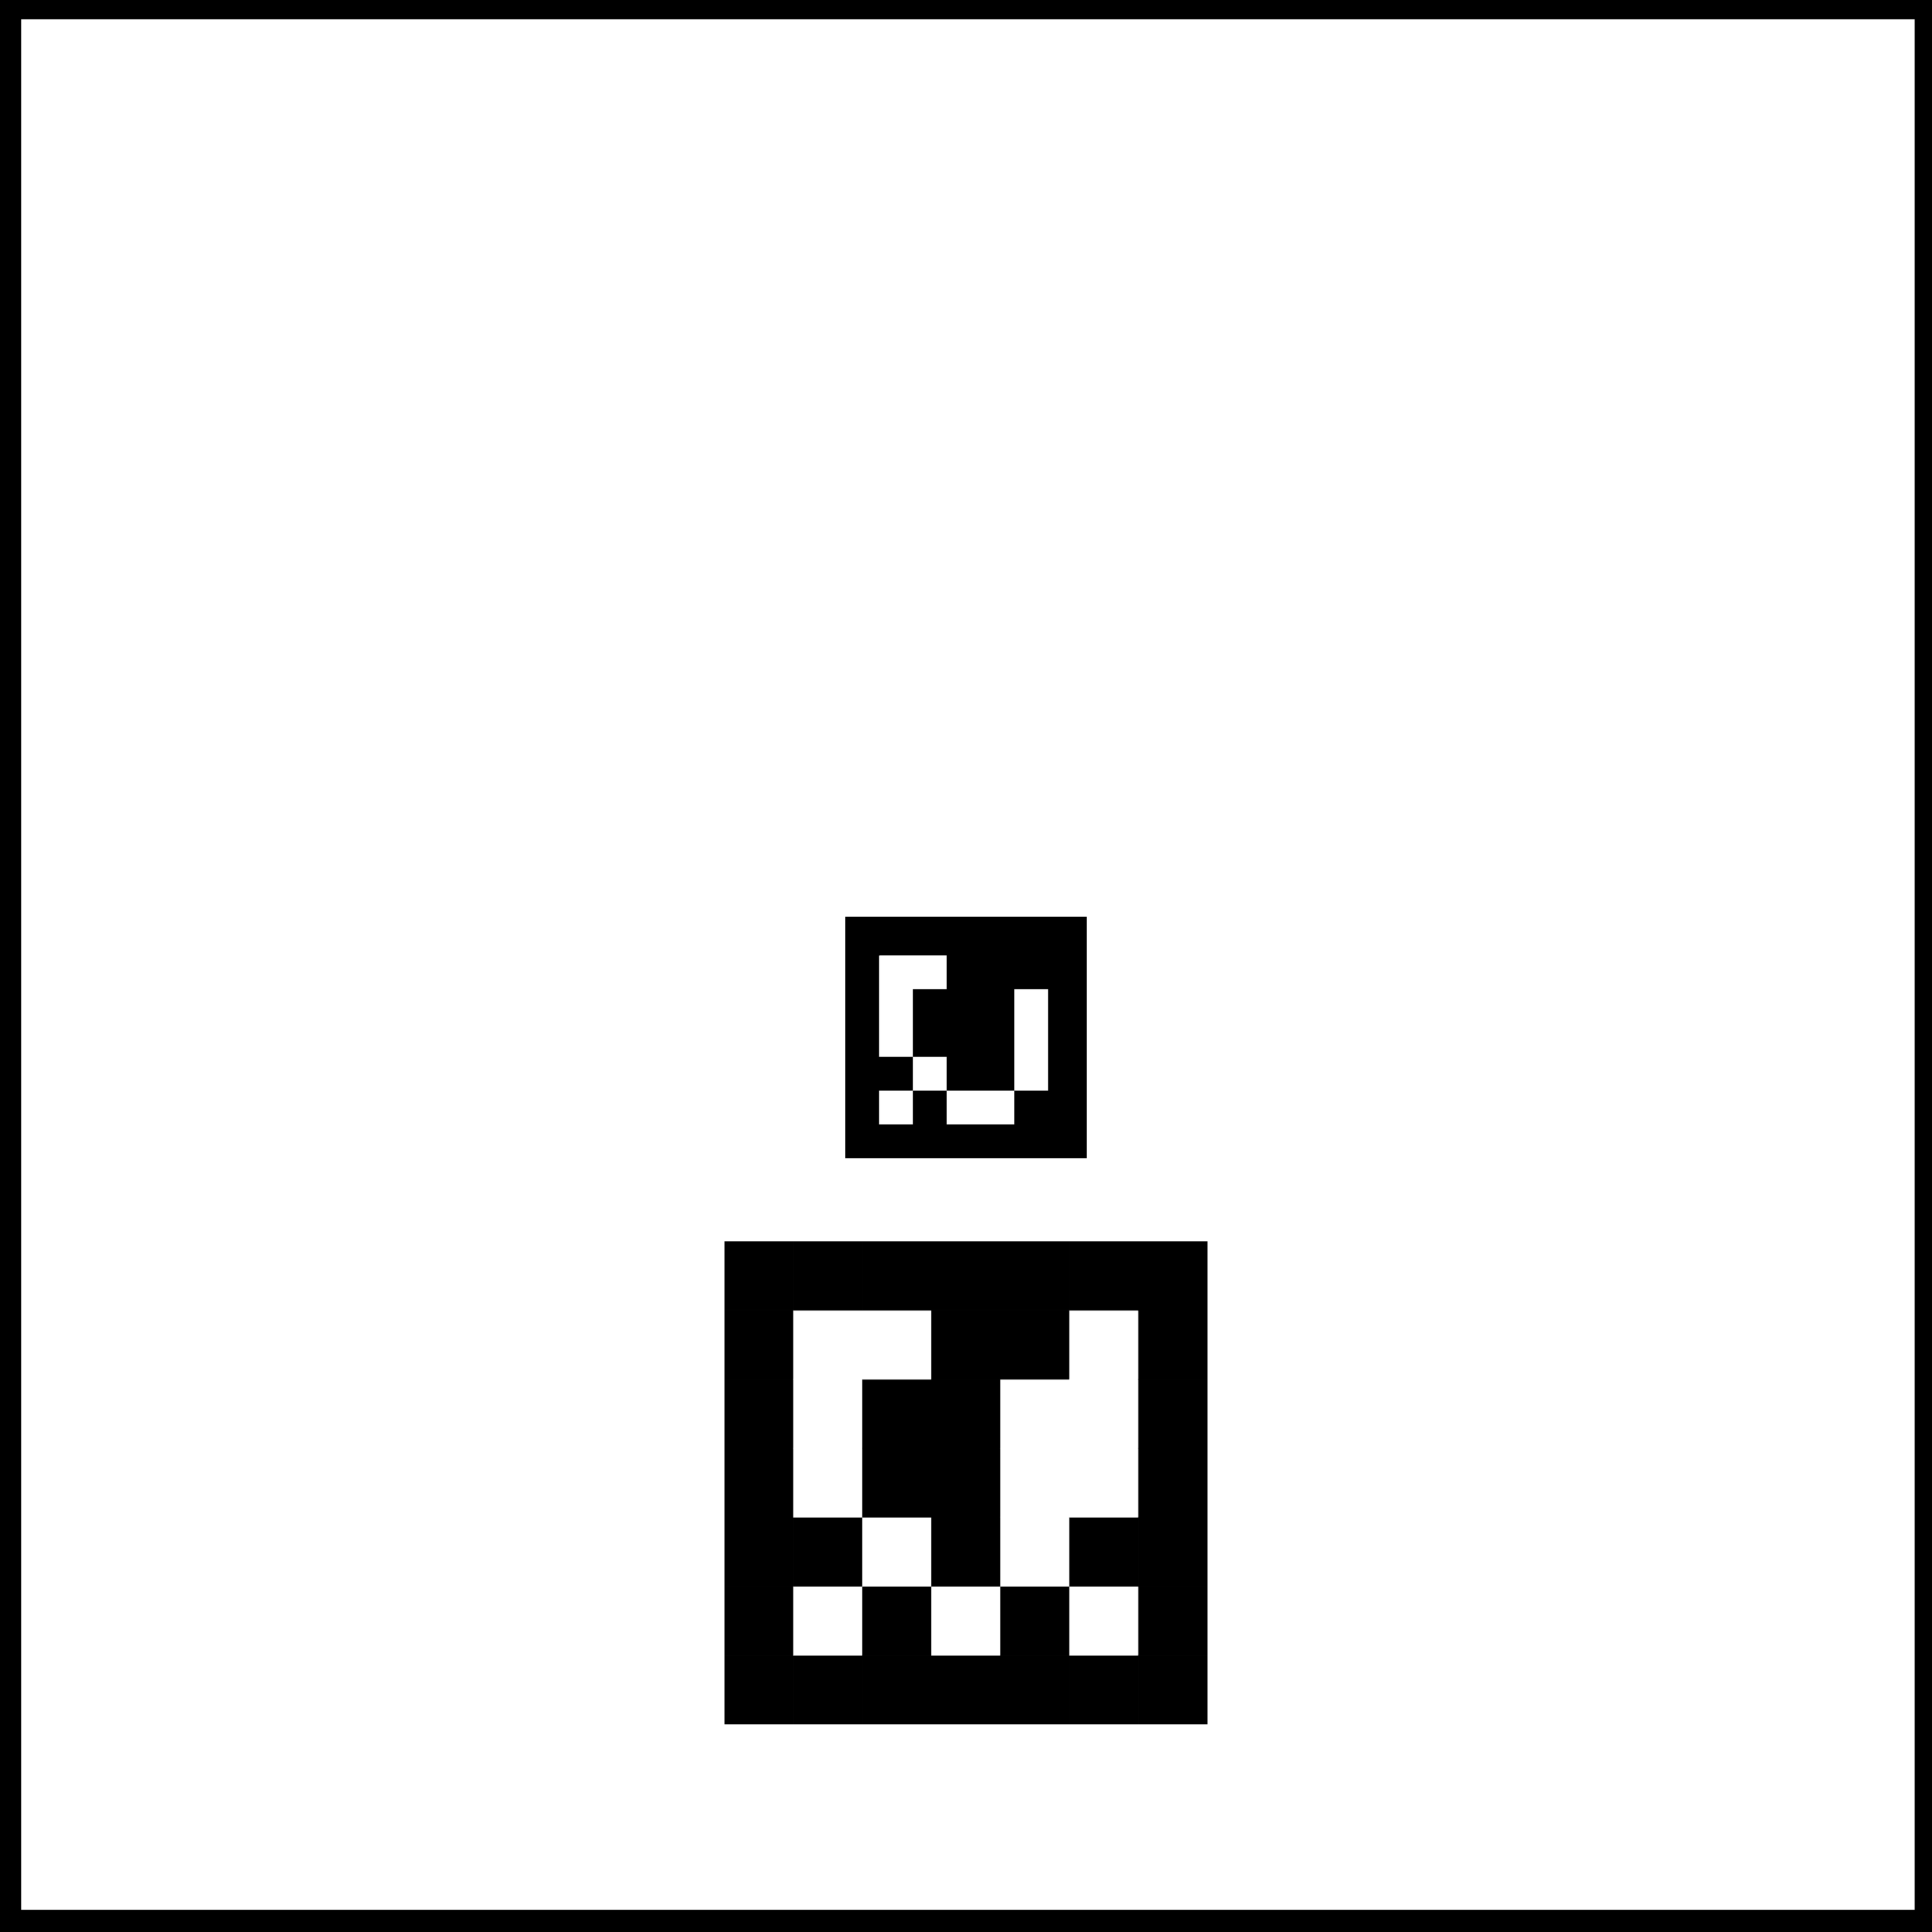
\includegraphics[width=0.5\textwidth]{img/tempbase.png}
    \caption{Design of the platform, we are using, in which the quadrotor must land on}
    \label{fig:tempplatform}
\end{figure}

\subsubsection{Implementation}
In the real world implementation we tried several different tag detector ROS packages, such as  RPG-April-Tags \cite{rpgapriltags} that uses the  AprilTags library \cite{apriltagslibrary}, AR-Sys \cite{arsys} and AR-Track-Alvar \cite{artrackalvar}.
All of them have some strengths and weaknesses:
\begin{itemize}
\item Light conditions: all these methods uses the edge based approach, so the results is similar in different light conditions.
\item Final pose: all trackers solve a PnP Problem to find the 6dof pose of the camera that minimize the reprojection error of the points on the image. The final result is the transformation between tag and camera. RPG-AprilTag has also the possibility to return a 4dof pose (perfect for our application), saving some computation.
\item Multiple tags: AR-Sys and AR-Track-Alvar possess the ability to directly track multiple objects and object composed by multiple tags.
\item Precision:we measure the error at $1m$ distance from the tag
\begin{itemize}
\item RPG-April-Tags: $\pm 1 pixel $ 
\item AR-Sys: $\pm 2 pixel $
\item AR-Track-Alvar: $\pm 1 pixel $
\end{itemize}
\item Frequency: on the quadrotor the performance of the three tracker where quite different
\begin{itemize}
\item RPG-April-Tags: $~1Hz$
\item AR-Sys: $~4Hz$
\item AR-Track-Alvar: $~1Hz$
\end{itemize}
\end{itemize}

\paragraph{AR-Sys}
In our final implementation we decided to use AR-Sys because its computational efficiency. AR-Sys is 3D pose estimation ROS package that uses ARUco marker boards \cite{Aruco2014}.\\
This package guarantees a good error correction in the identification of a specific tag, and, more interesting for our application, a solution to the occlusion problem using multiple markers. This package can identify the pose of boards composed by multiple tags considered as a single unit. This guarantees more stable pose estimates and robustness to occlusions. The board is defined in an XML file where all the tag are listed with an ID and the relative position w.r.t. the master tag (the first in the list) that defines the center of the cumulative tag, the pose of the camera is given with respect to this tag. 

\begin{figure}[!htbp]
  \centering
   \begin{subfigure}[b]{0.45\textwidth}
        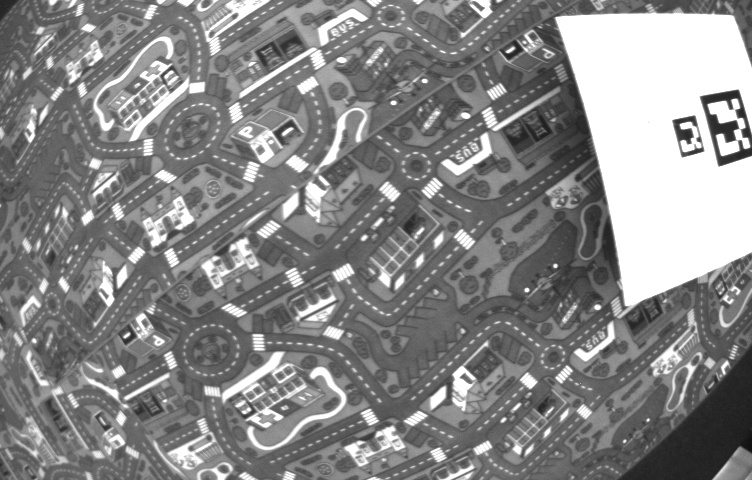
\includegraphics[width=\textwidth]{img/frame0.jpg}
        \caption{If we are far from the moving platform we have to use the big tag to identify the base.}
        \label{fig:one}
   \end{subfigure}\hfill
   \begin{subfigure}[b]{0.45\textwidth}
        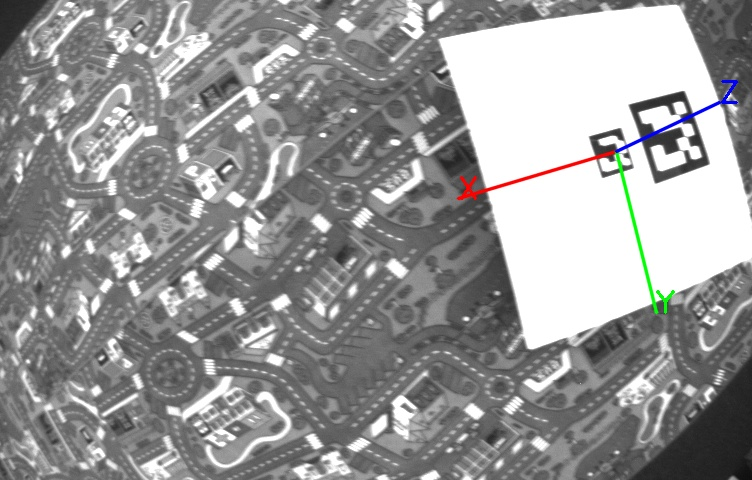
\includegraphics[width=\textwidth]{img/frame1.jpg}
        \caption{So only when the bigger square is inside the FOV we can detect the center of the base correctly.}
        \label{fig:two}
   \end{subfigure}
   
   \begin{subfigure}[b]{0.45\textwidth}
        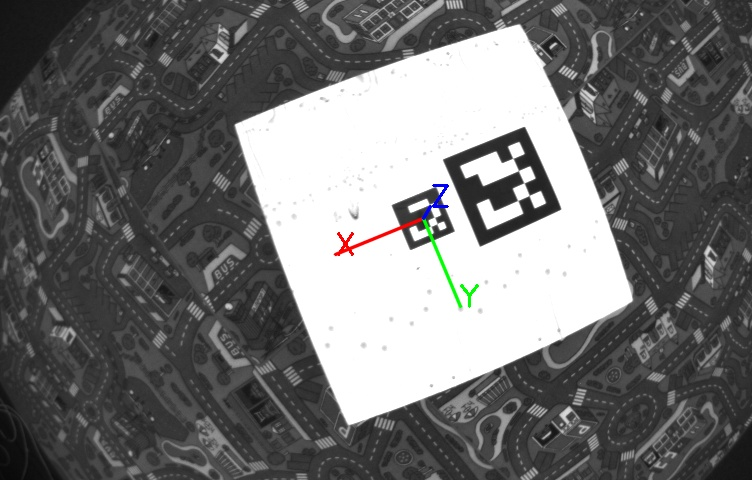
\includegraphics[width=\textwidth]{img/frame2.jpg}
        \caption{When both the tags are visible we use all the information to have the best position of the master tag.}
        \label{fig:three}
   \end{subfigure}\hfill
    \begin{subfigure}[b]{0.45\textwidth}
        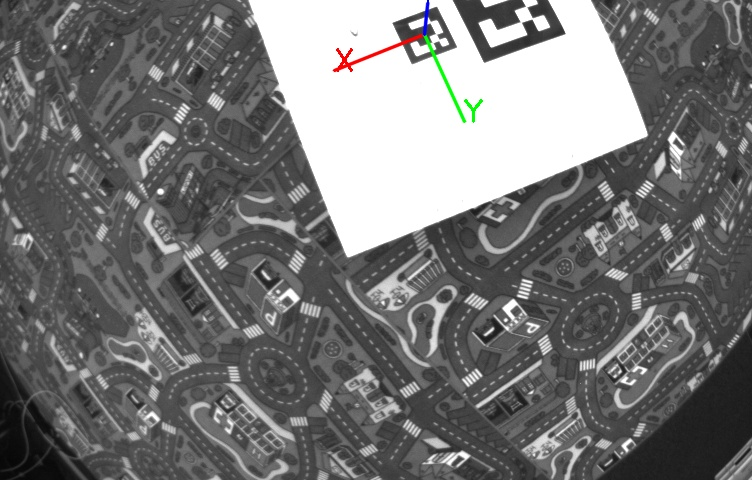
\includegraphics[width=\textwidth]{img/frame3.jpg}
        \caption{Even if we lose one or more tag of the board we still have the pose estimation of the center.}
        \label{fig:four}
   \end{subfigure}
   
    \begin{subfigure}[b]{0.45\textwidth}
        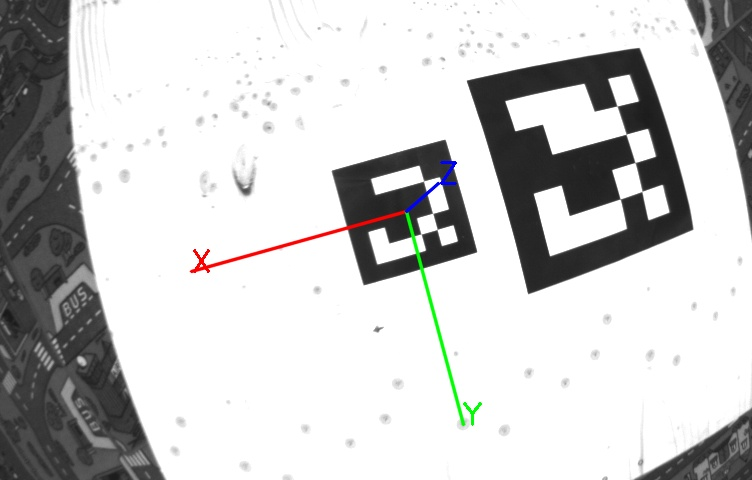
\includegraphics[width=\textwidth]{img/frame4.jpg}
        \caption{The landing maneuver is performed to be finished over the central tag. So while we are landing the bigger and further tags leave the FOV.  }
        \label{fig:five}
   \end{subfigure}\hfill
    \begin{subfigure}[b]{0.45\textwidth}
        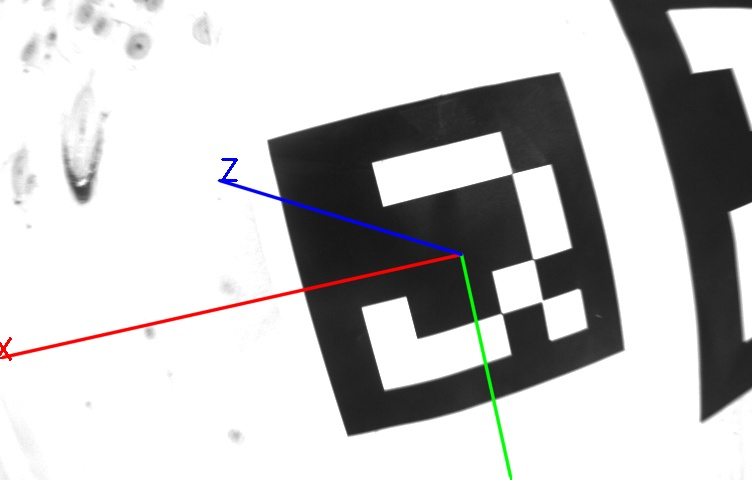
\includegraphics[width=\textwidth]{img/frame5.jpg}
        \caption{At the end only the central tag is entirely on the FOV, so this tag must be little in order to have the possibility to track it until the very end.}
        \label{fig:six}
   \end{subfigure}
   
  \caption{A sequence of images where the AR-Tag over the base is detected. The coordinate system related to the moving platform has its origin on the master tag. The landing is performed over this tag.}
  \label{fig:arsys}
\end{figure} 


\subsection{Covariance Estimation}
In the practical implementation of the Kalman Filter is crucial to find a good estimate of the noise covariance matrices $Q_k$ and $R_k$ for the prediction and the measurement steps. \\
When a manual tuning is required, these matrices are considered diagonal, such as each component of the state vector is corrupted by a Gaussian processes that is independent with respect to all the other coordinates. It is easy to give a physical interpretation to the components of the diagonal, so it is easy to find correct values for them.\\
The equations \ref{eq:ekf1} is the general matrix formulation of the system corrupted by a multivariable Gaussian noise $\boldsymbol{w}_k$. Now, if we consider the covariance matrix $Q_k$ diagonal we can split the equation  \ref{eq:ekf1} into:
\begin{align}
{\begin{bmatrix}
\dot{x}_k^1 \\[10pt]
\dot{x}_k^2 \\[10pt]
\vdots \\[10pt]
\dot{x}_k^n
\end{bmatrix}}=
{\begin{bmatrix}
 f_1(\boldsymbol{x}_{k-1},\boldsymbol{u}_k) \\[10pt]
f_2(\boldsymbol{x}_{k-1},\boldsymbol{u}_k)  \\[10pt]
\vdots \\[10pt]
f_n(\boldsymbol{x}_{k-1},\boldsymbol{u}_k) 
\end{bmatrix}} 
+ 
{\begin{bmatrix}
w_k^1 \\[10pt]
w_k^2 \\[10pt]
\vdots \\[10pt]
w_k^n
\end{bmatrix}}
\end{align}
where $w_k^i$ is a scalar Gaussian random variable with variance $q_k^i$. This variance can now be directly related to the error that is generally computed when the variable is predicted with the theoretical model.\\
For the error update equation \ref{eq:ekf2} the concept is the same: 
\begin{align}
{\begin{bmatrix}
z_k^1 \\[10pt]
z_k^2 \\[10pt]
\vdots \\[10pt]
z_k^m
\end{bmatrix}}=
{\begin{bmatrix}
 h_1(\boldsymbol{x}_{k-1}) \\[10pt]
h_2(\boldsymbol{x}_{k-1})  \\[10pt]
\vdots \\[10pt]
h_m(\boldsymbol{x}_{k-1}) 
\end{bmatrix}} 
+ 
{\begin{bmatrix}
v_k^1 \\[10pt]
v_k^2 \\[10pt]
\vdots \\[10pt]
v_k^m
\end{bmatrix}}
\end{align}
with $v_k^i$ scalar Gaussian noise with variance $r_k^i$. This variance is even more understandable and it is related on the actual error that we are making while measuring the component $z_k^i$ due to measurement limitations.\\
In our case the measures are \ref{eq:realmeasure} and they are computed with the methods described in the previous section. To estimate the variance of the measure we must start from the error computed in the image when we detect the pose of the platform and propagate the correspondent covariance in the real world. The propagation of uncertainty is the effect of variables'  uncertainties on the uncertainty of a function based on them.\\
Supposed that in the equation \ref{eq:ekf2} $\boldsymbol{z}_k$ is not a direct measure of $\boldsymbol{x}_{k}$
but is a function of other variables $\boldsymbol{\gamma}_k$, such as:
\begin{align}
h(\boldsymbol{x}_{k}) = g(\boldsymbol{\gamma}_k)
\end{align}
Then we can easily estimate the measurement error (variance) that we have computed during the observation of  $\boldsymbol{\gamma}_k$, but we need the correspondent error for the measures $ g(\boldsymbol{\gamma}_k)$.\\

In the linear case 
\begin{align}
g(\boldsymbol{\gamma}_k) = \mathrm {A}\boldsymbol{\gamma}_k
\end{align}
The covariance matrix $\mathrm {\Sigma }_g$ of $g$ is related to $\mathrm {\Sigma }_{\boldsymbol{\gamma}}$, the covariance of the variable $\boldsymbol{\gamma}$, by the equation:
\begin{align}
\begin{split}
Cov(g) &= Cov(\mathrm {A}\boldsymbol{\gamma}_k) = \mathrm {A}Cov(\boldsymbol{\gamma}_k)\mathrm {A} ^{\top} \\ 
\mathrm {\Sigma }_g &=\mathrm {A} \mathrm {\Sigma }_{\boldsymbol{\gamma}}\mathrm {A} ^{\top}
\end{split}
\end{align}

If the function $g$ is a set of non-linear combination of the variables $\gamma_i$,  it must be linearized by approximation to a first-order Taylor series expansion:
\begin{align}
g_{i}(\boldsymbol{\gamma}_{k}) \approx g_{i}(\tilde{\boldsymbol{\gamma}}_{k})+\sum _{j}^{n}{\frac  {\partial g_{i}}{\partial {\gamma_{j}}}}\Big|_{\tilde{\gamma}_k^{j}}(\gamma_k^{j}-\tilde{\gamma}_k^{j})
\end{align}
where ${\frac  {\partial g_{i}}{\partial {\gamma_{j}}}}\Big|_{\tilde{\gamma}_k^{j}}$ denotes the partial derivative of $g_i$ with respect to the j-th variable, evaluated at the measured component $\tilde{\gamma}_k^{j}$.\\
In matrix notation the first-order Taylor series expansion is:
\begin{align}
g(\boldsymbol{\gamma}_{k}) \approx g(\tilde{\boldsymbol{\gamma}}_{k})+J\Big|_{\tilde{\gamma}_k}(\gamma_k-\tilde{\gamma}_k)
\end{align}
where $J$ is the Jacobian matrix. Since $g(\tilde{\boldsymbol{\gamma}}_{k})$ is a constant it does not contribute to the error on $g$, so the propagation of the error can be approximate with the linear case where $A = J$:
\begin{align}
{\displaystyle \mathrm {\Sigma }_g\approx \mathrm {J} \mathrm {\Sigma }_{\boldsymbol{\gamma}}\mathrm {J} ^{\top}} 
\label{eq:errorpropag}
\end{align}

In our case to have the final measure $\boldsymbol{z}_k$  in the 3D real world coordinate system, we start from a measure in pixel in the image coordinate system. We have the function $g : \mathrm{R}^{6 \times 6} \to \mathrm{R}^{2 \times 2} $ that is converting the real world coordinate in image coordinate, and its Jacobian matrix $J \in \mathrm{R}^{2 \times 6} $.\\
Now to calculate the covariance of the final pose estimate, $\mathrm {\Sigma }_{RW} \in \mathrm{R}^{6 \times 6} $, from the covariance of the image position  $\mathrm {\Sigma }_{I} \in \mathrm{R}^{2 \times 2} $, we need to invert the equation \ref{eq:errorpropag}:

\begin{align}
{\displaystyle \mathrm{\Sigma}_{RW} = ( \mathrm{J}^{\top} \mathrm{\Sigma }_{I} \mathrm{J})^{-1} } 
\label{eq:errorpropag}
\end{align}

In our implementation we do not have a single function $g$ from image pixel $(u,v)$ to 3D coordinate $(x,y,z,\theta)$. The passage from image to 6dof pose is done using the openCV function $solvePnP$ \cite{opencv_library} that returns a pose expressed as 3D coordinates $(x,y,z)$ and Rodrigues orientation  \cite{belongie1999rodrigues}. To convert the orientation in Euler angles we convert the Rodrigues angles into a rotation matrix and the rotation matrix into finally $(roll,pitch,yaw)$ notation:
\begin{align}
\begin{split}
J_{solvePnP} &= J_0 = \Big[ \frac  {\partial g}{\partial rodrigues},  \frac {\partial g}{\partial xyzpos} \Big] \\
J_{rodriguesToR} &= J_1 =  \frac  {\partial rodrigues}{\partial R}, \\
J_{RToEuler} &= J_2 =  \frac  {\partial R}{\partial euler}, \\
J_{Final} &= J = \Big[ \frac  {\partial g}{\partial euler},  \frac {\partial g}{\partial xyzpos} \Big]  = J_{0}{\begin{bmatrix}
J_{1}J_{2} & 0 \\[10pt]
0 & I 
\end{bmatrix}}
\end{split}
\end{align}
 

\section{Results of the tracking}
Several experiments were performed both in simulation and in the real world to evaluate the performance of the state estimation.
\subsection{From high altitude}
We are not requiring that the state estimation from high altitude is very precise, we need a rough estimation of the position of the platform. With the designed  EKF we obtain a reliable estimation with an RMSE error in both $x,y$ coordinate of $40cm$

\begin{figure}[!htbp]
  \centering
  \begin{subfigure}[b]{0.5\textwidth}
        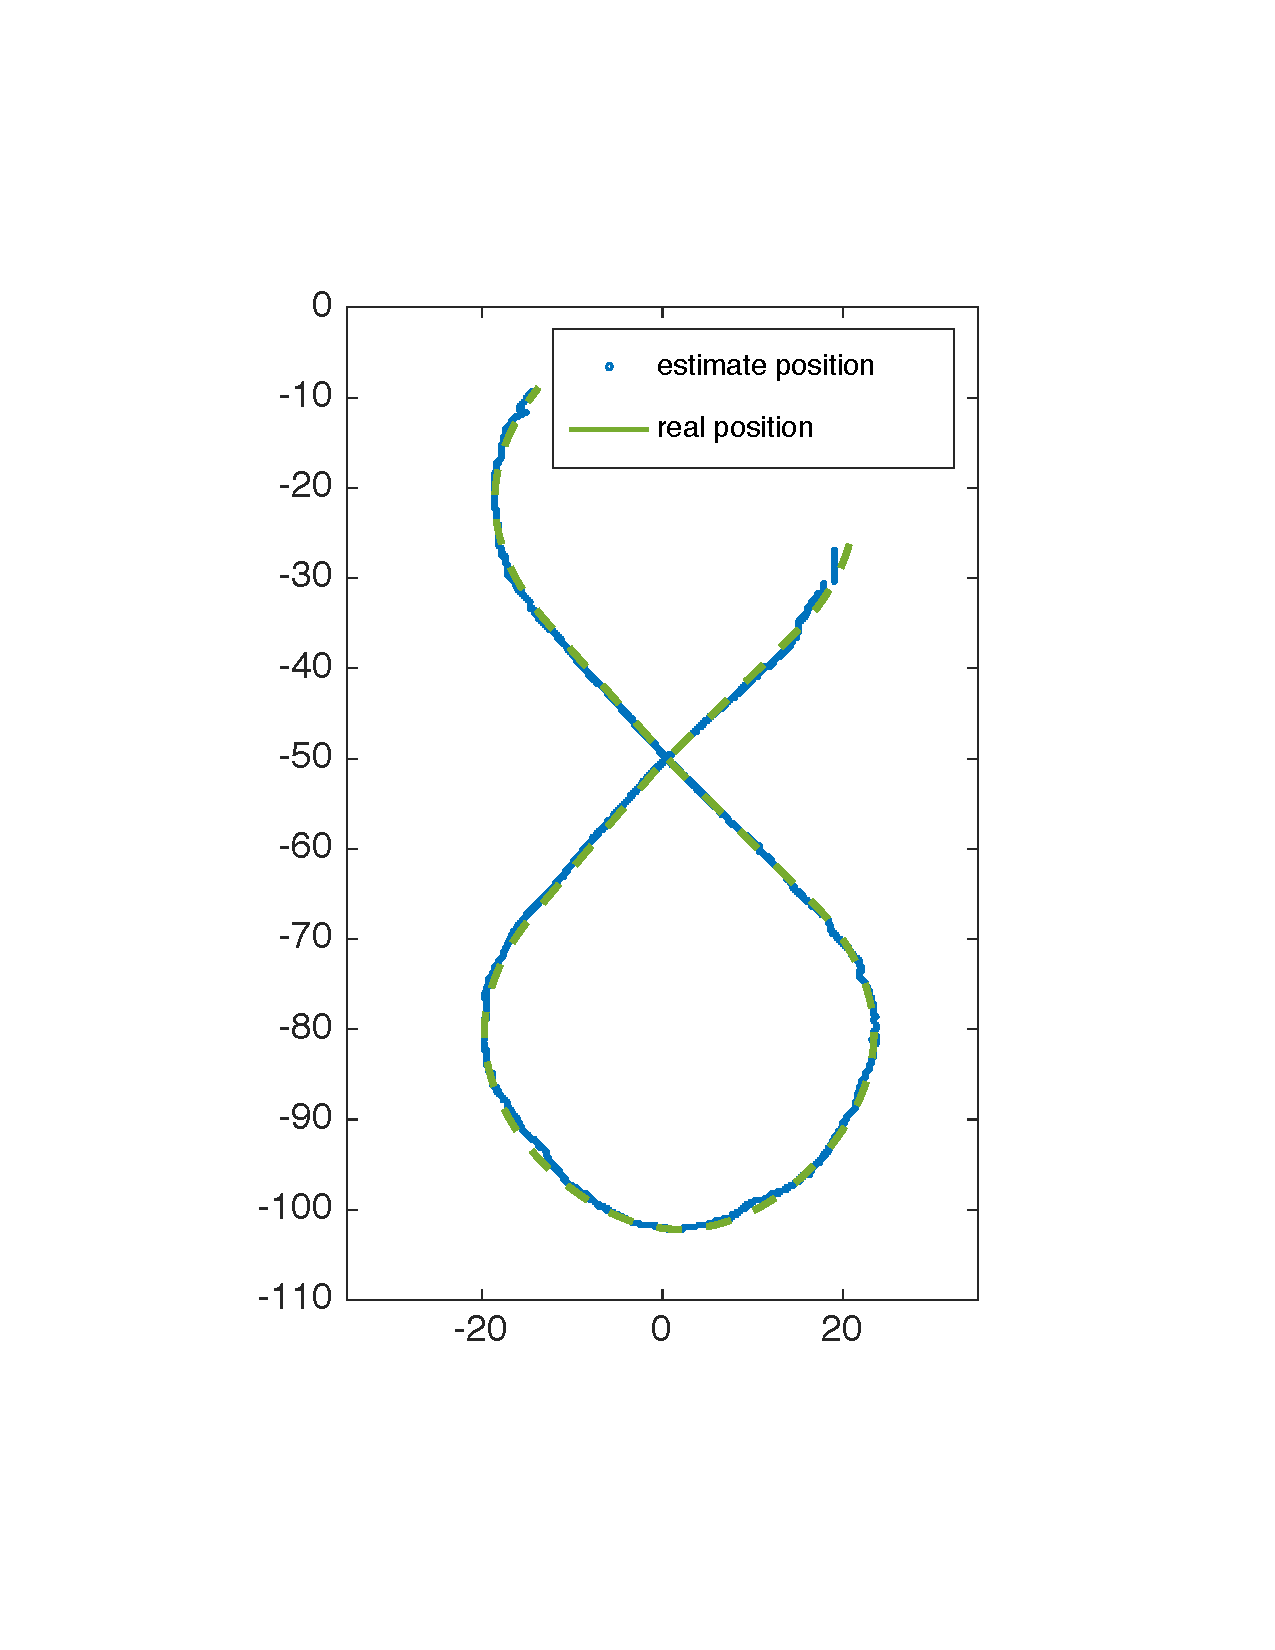
\includegraphics[width=\textwidth]{img/high_altitude_error_xy.pdf}
        \caption{Trajectory}
        \label{fig:one}
   \end{subfigure} \\
   \begin{subfigure}[b]{0.45\textwidth}
        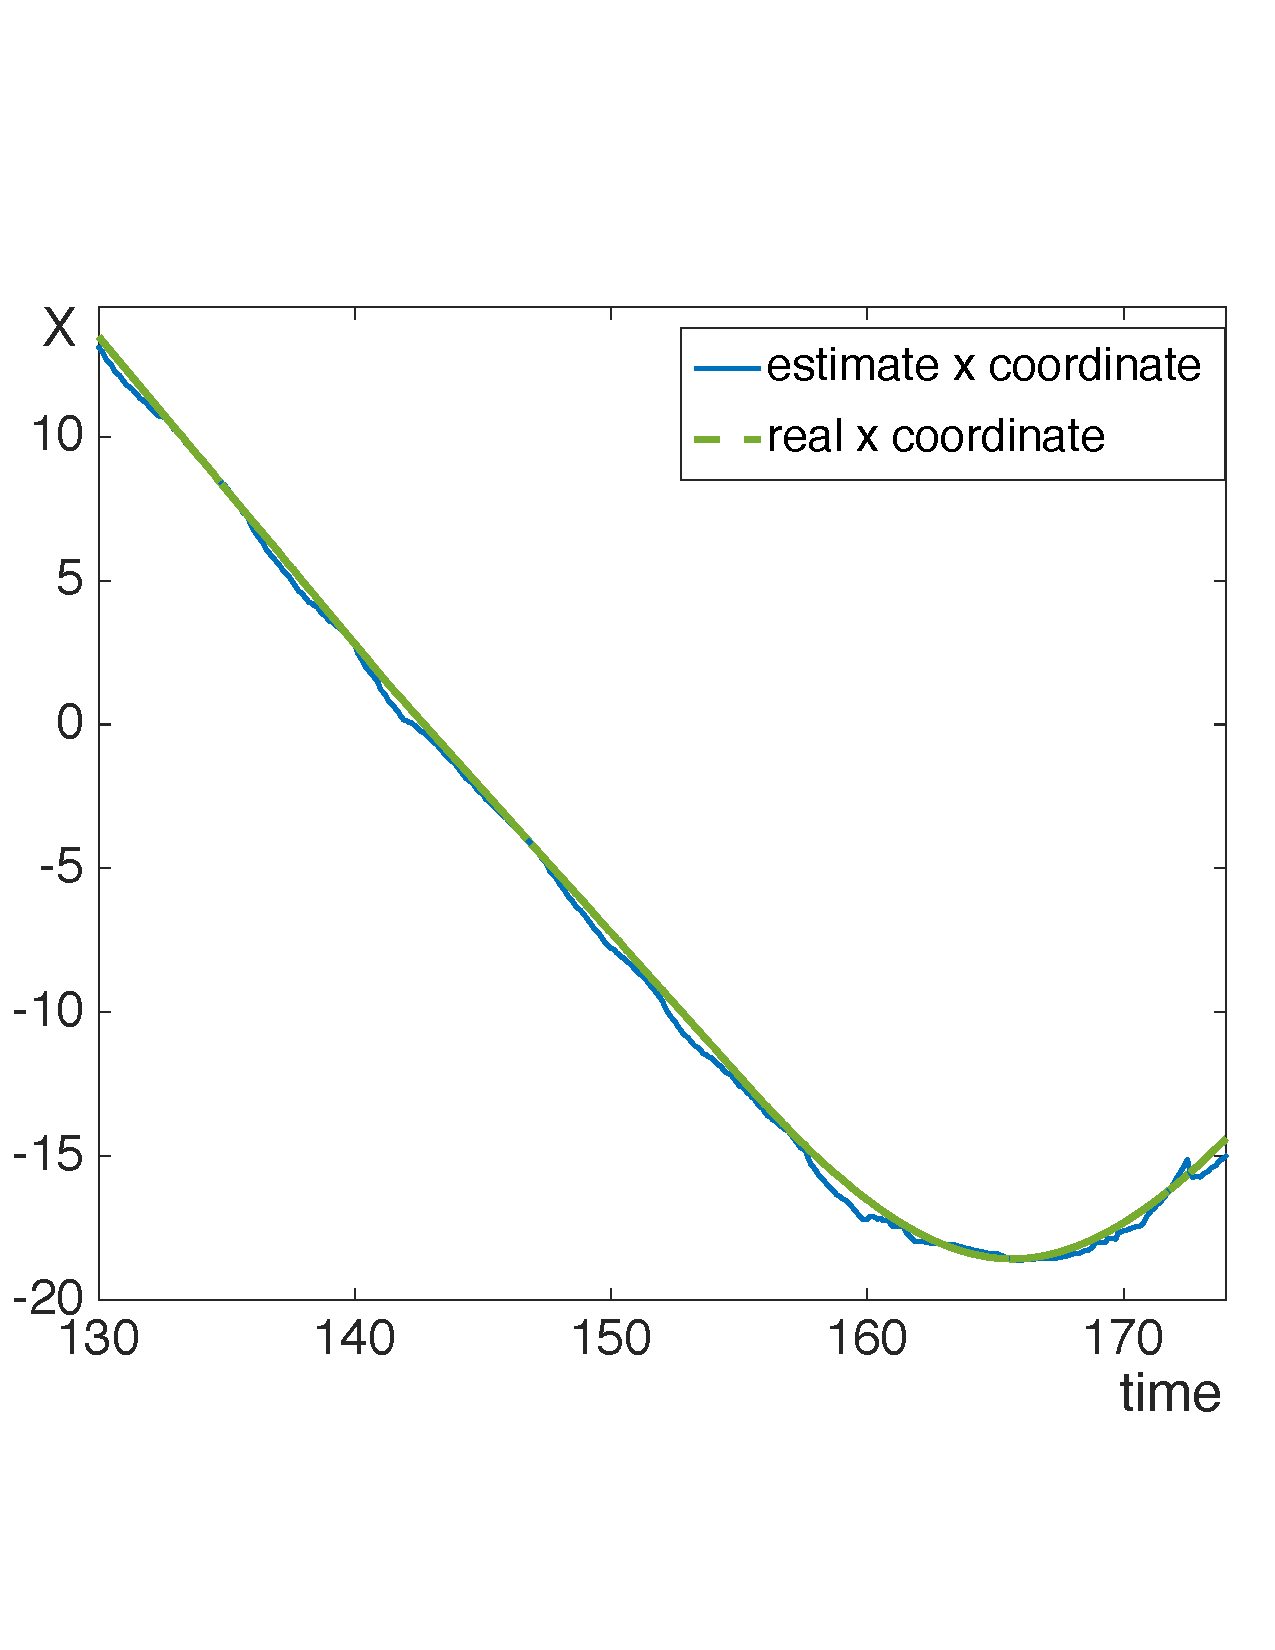
\includegraphics[width=\textwidth]{img/high_altitude_error_x.pdf}
        \caption{x }
        \label{fig:one}
   \end{subfigure}\hfill
   \begin{subfigure}[b]{0.45\textwidth}
        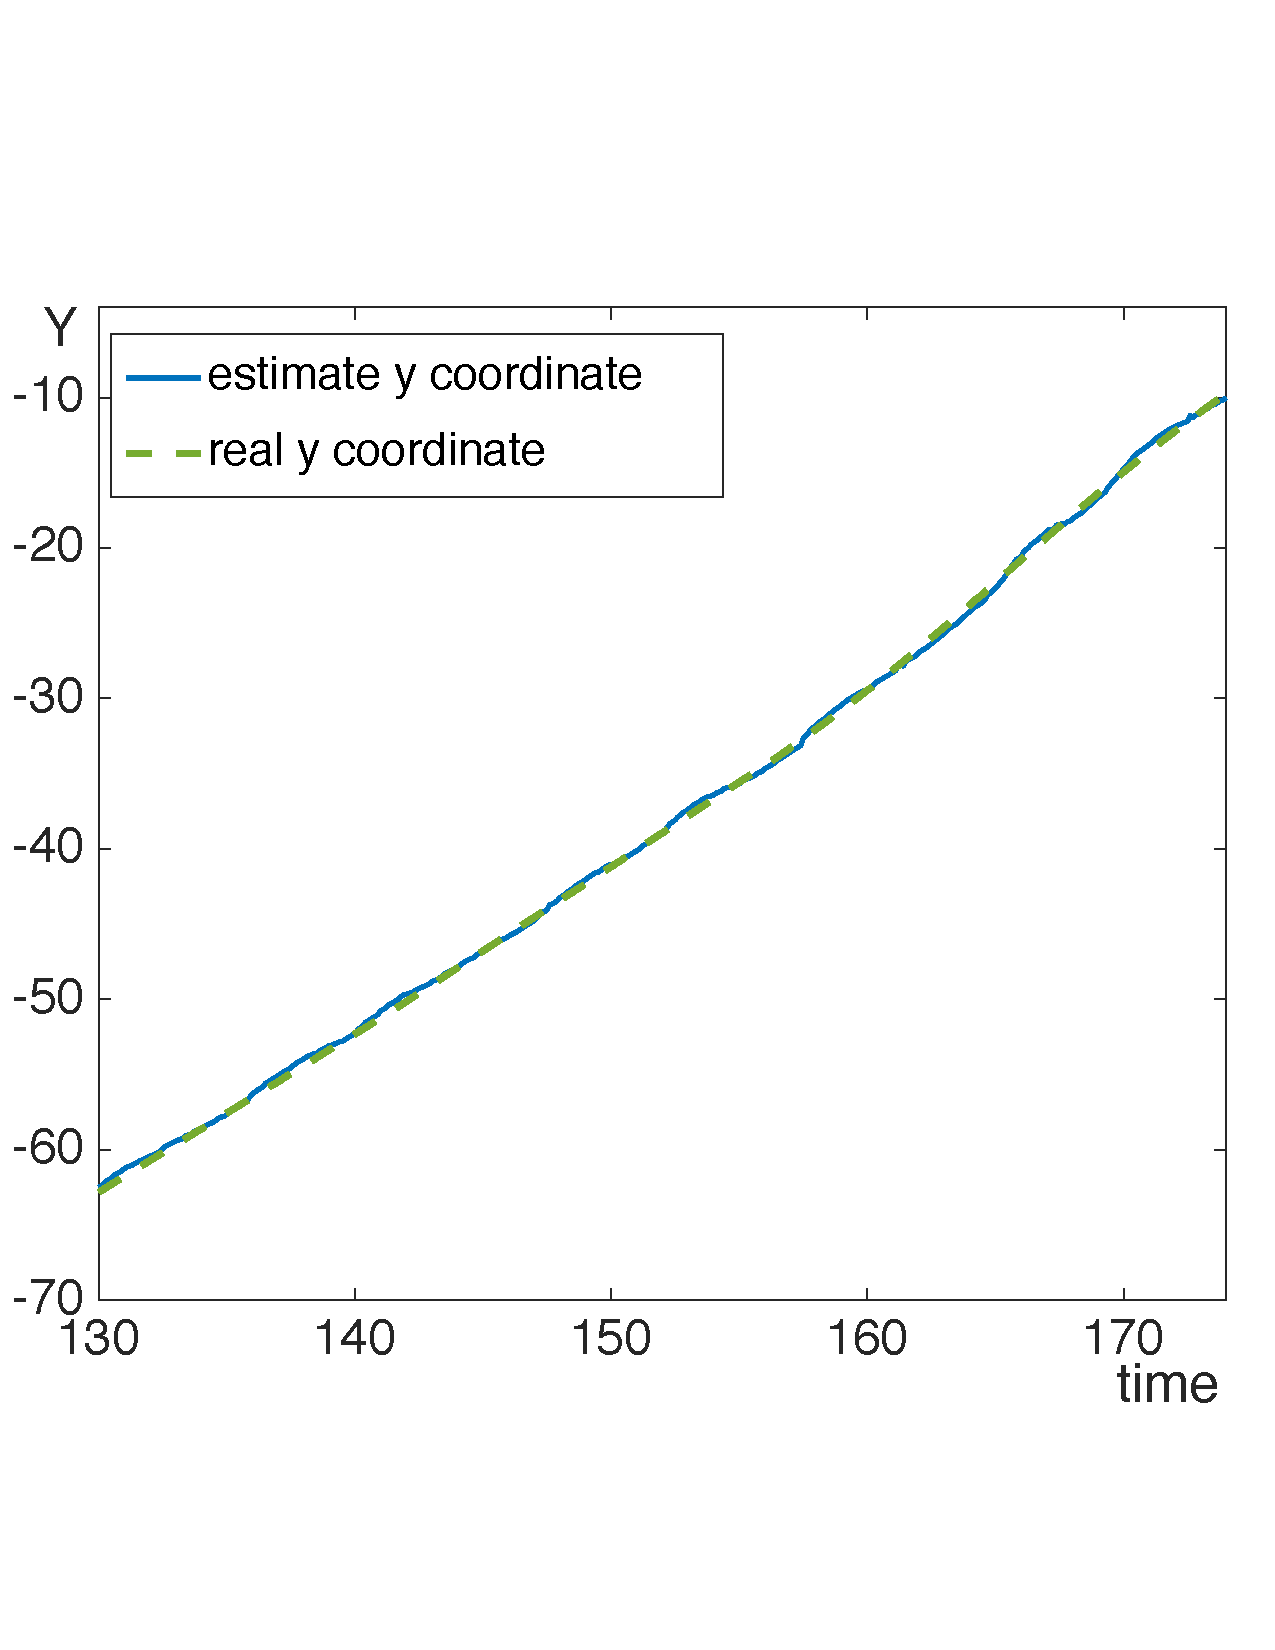
\includegraphics[width=\textwidth]{img/high_altitude_error_y.pdf}
        \caption{y}
        \label{fig:two}
   \end{subfigure}
  \caption{Comparison}
  \label{fig:ekf_high_altitude_comparison}
\end{figure} 

\begin{figure}[!ht]
    \centering
    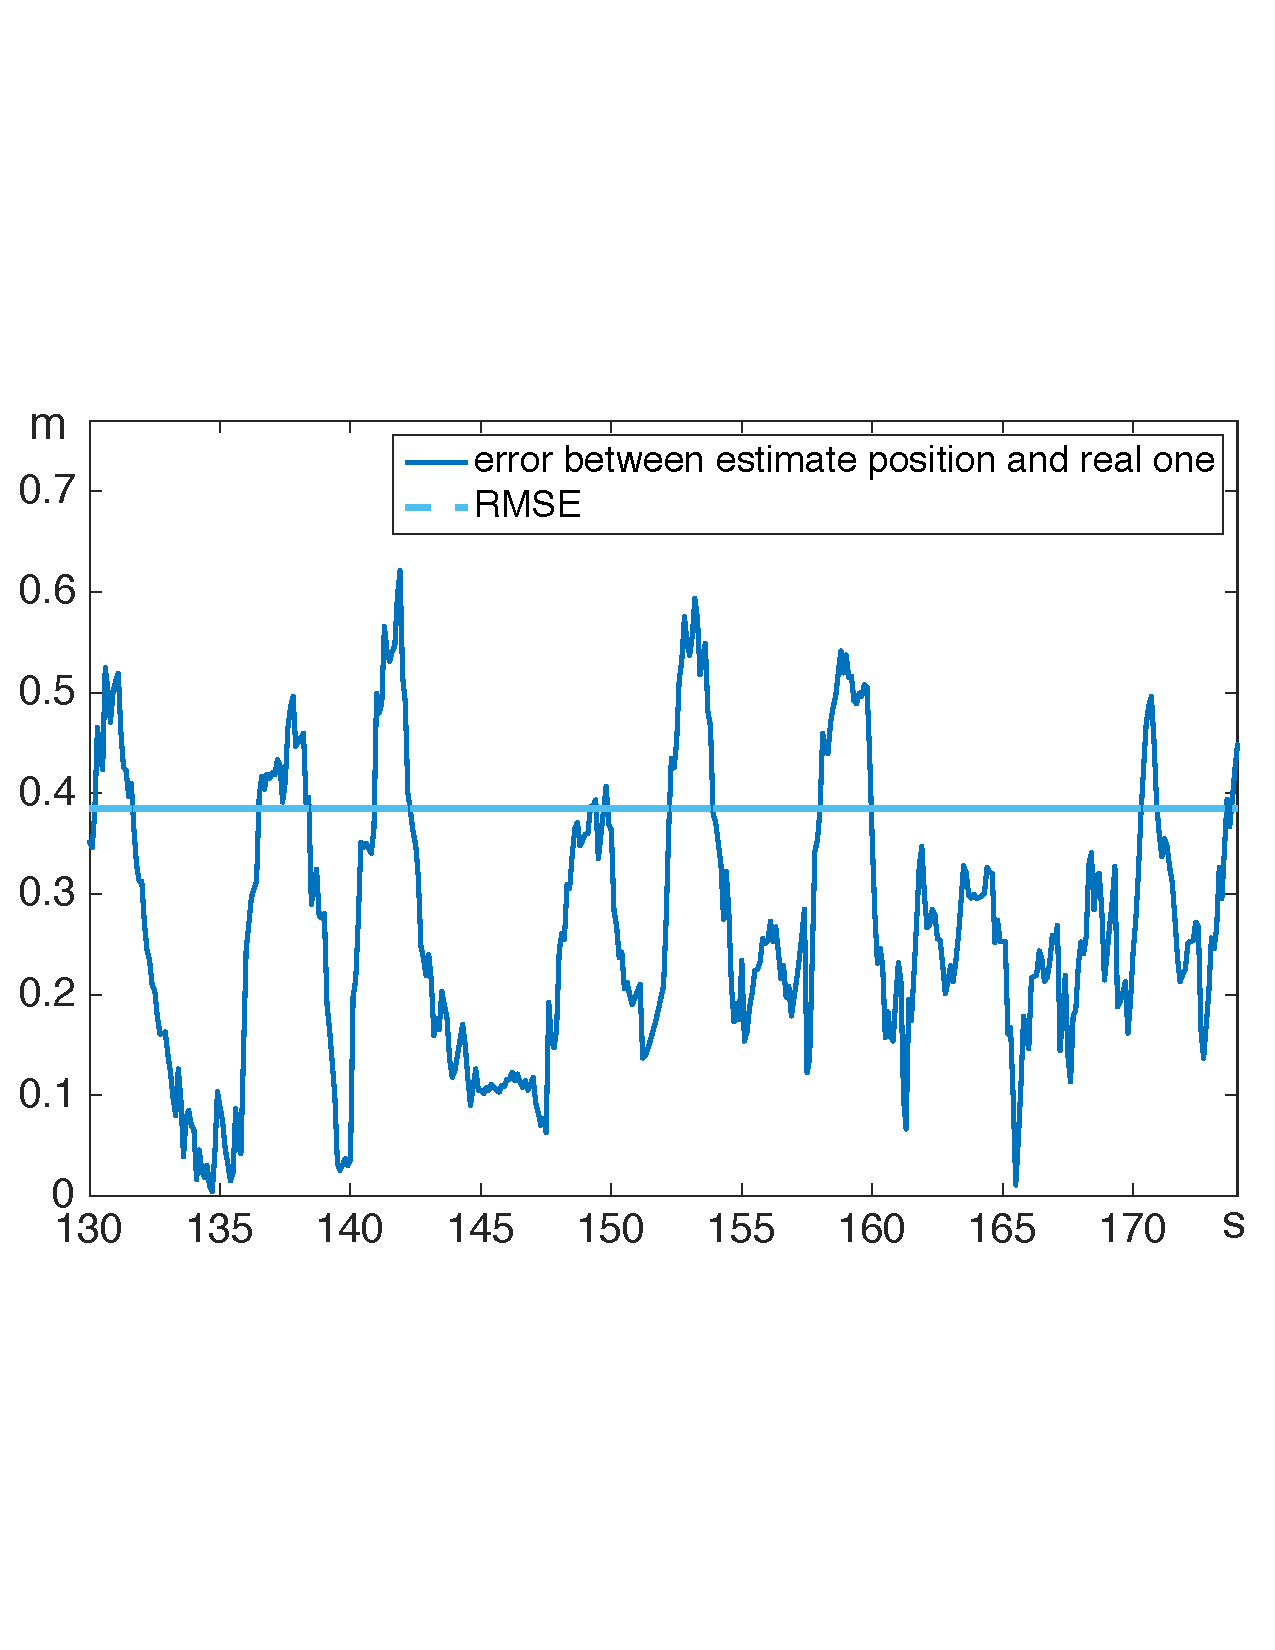
\includegraphics[width=0.8\textwidth]{img/high_altitude_error.pdf}
      \caption{error}
    \label{fig:ekf_high_altitude_error}
\end{figure}

\subsection{From low altitude}
Very accurate pose estimation is obtain when the AR tags are used. Generally the error in the $x,y$ coordinate is less then $5cm$ while in the $z$ direction is about $3cm$.
\begin{figure}[!htbp]
  \centering
   \begin{subfigure}[b]{0.45\textwidth}
        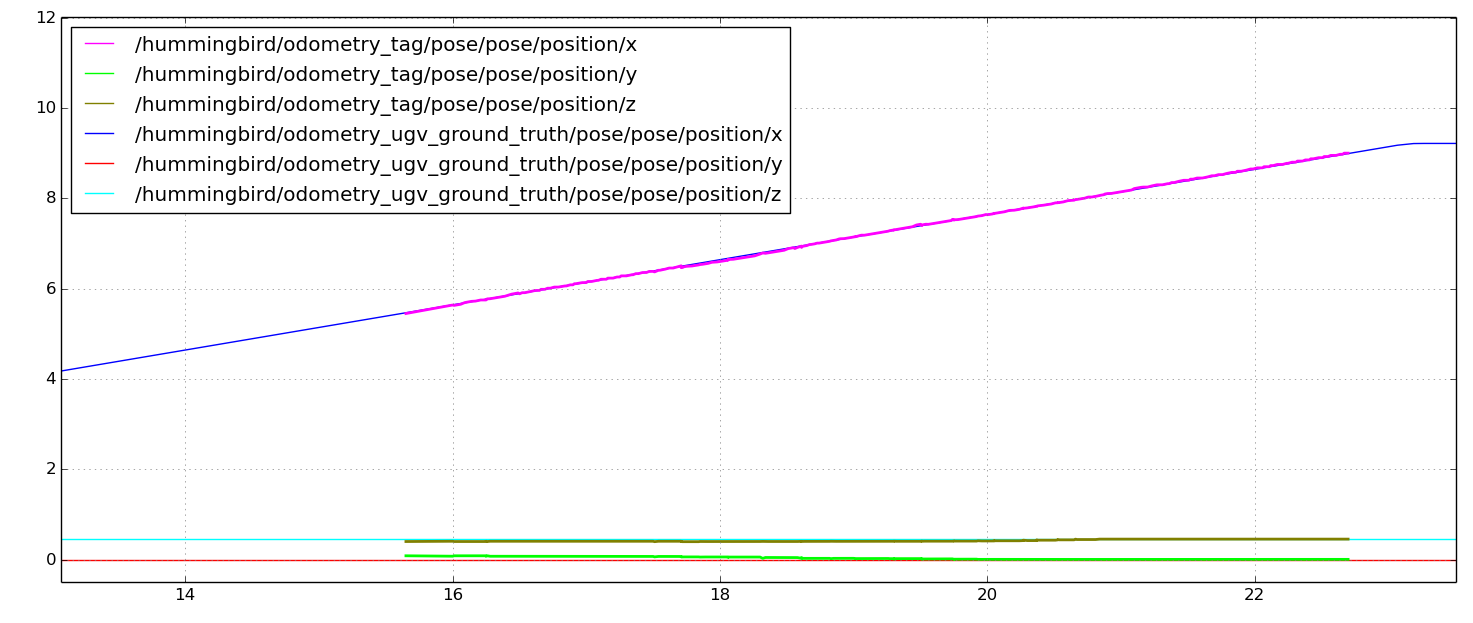
\includegraphics[width=\textwidth]{img/position_simulation_hot_init.png}
        \caption{Position }
        \label{fig:one}
   \end{subfigure}\hfill
   \begin{subfigure}[b]{0.45\textwidth}
        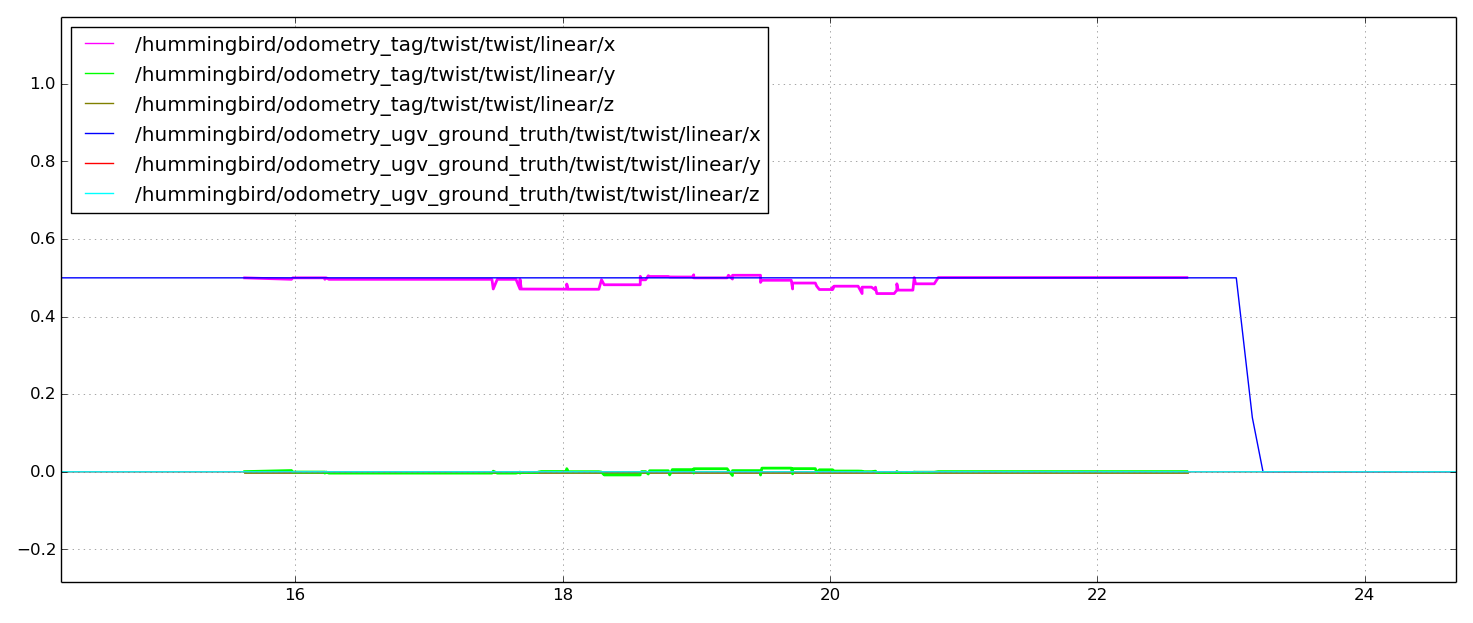
\includegraphics[width=\textwidth]{img/velocity_simulation_hot_init.png}
        \caption{Velocity}
        \label{fig:two}
   \end{subfigure}
  \caption{Simulation test. Comparison between estimate position and velocity with the ground truth values. The velocity is initialized with the right value.}
  \label{fig:ekf_simulation_hot_init}
\end{figure} 

\begin{figure}[!htbp]
  \centering
   \begin{subfigure}[b]{0.45\textwidth}
        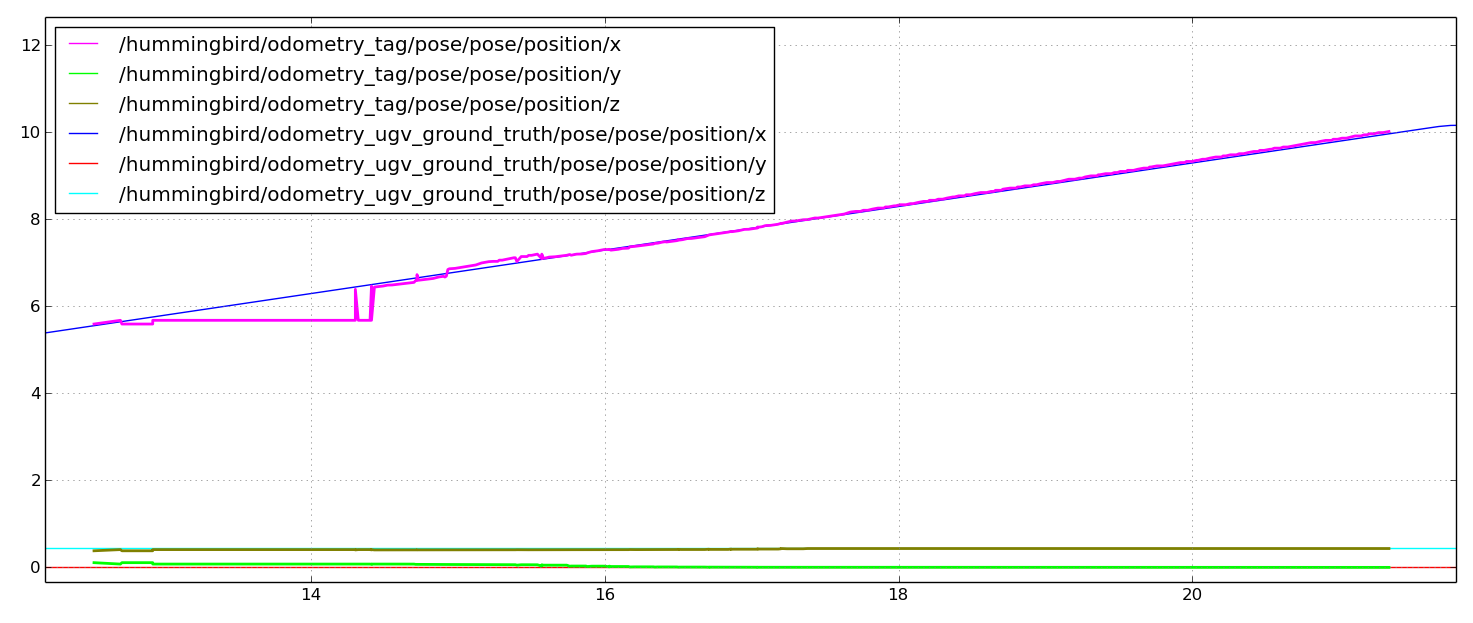
\includegraphics[width=\textwidth]{img/position_simulation.png}
        \caption{Position }
        \label{fig:one}
   \end{subfigure}\hfill
   \begin{subfigure}[b]{0.45\textwidth}
        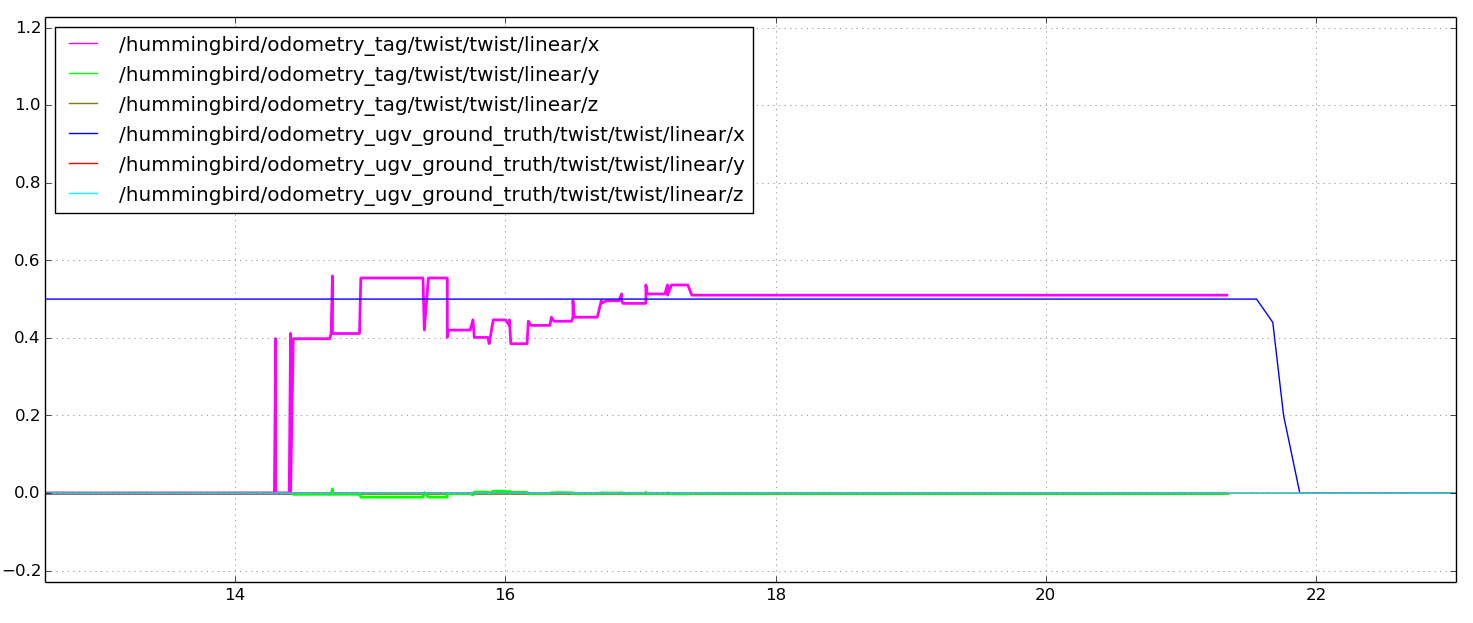
\includegraphics[width=\textwidth]{img/velocity_simulation.png}
        \caption{Velocity}
        \label{fig:two}
   \end{subfigure}
  \caption{Simulation test. Comparison between estimate position and velocity with the ground truth values. The velocity is initialized with 0 value. In this case the filter needs some time to converge to the right value of velocity.}
  \label{fig:ekf_simulation_hot_init}
\end{figure}

\begin{figure}[!ht]
    \centering
    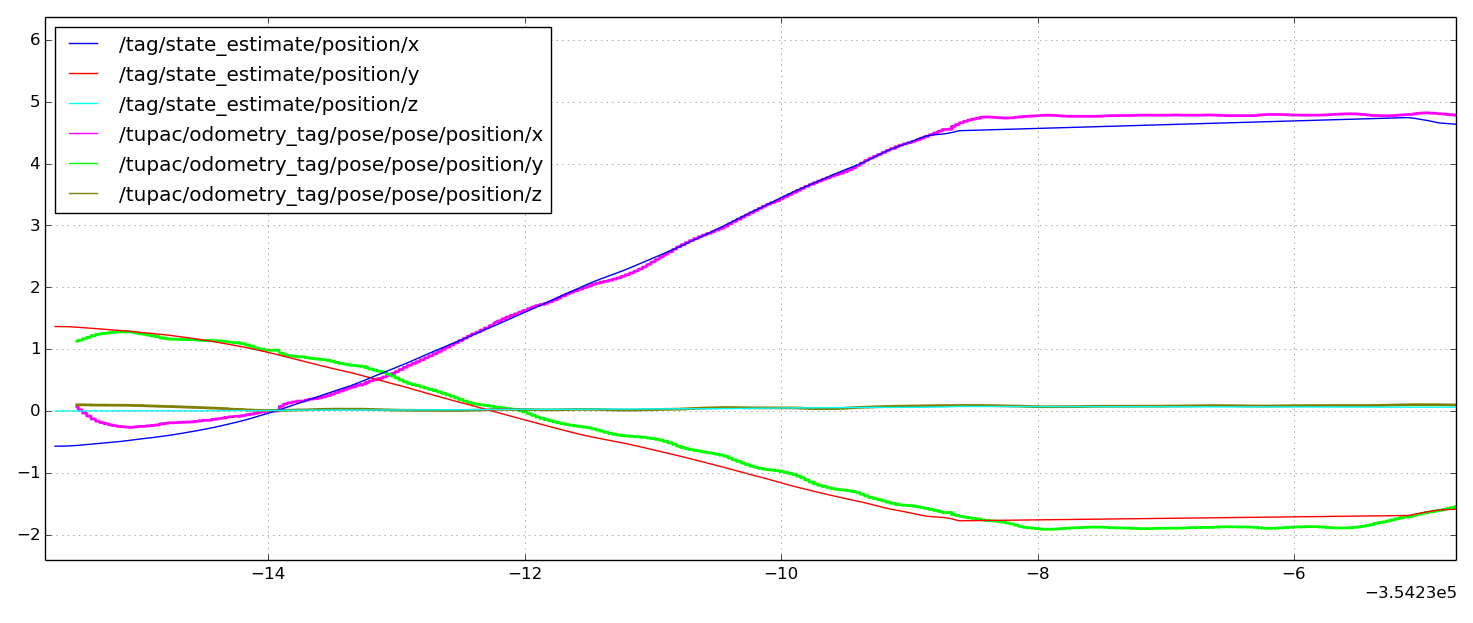
\includegraphics[width=0.97\textwidth]{img/position_real_world.png}
    \caption{Real world test. Comparison between estimate position and ground truth for a platform moving at $1\frac{m}{s}$}
    \label{fig:ekf_position_real}
\end{figure}

\begin{figure}[!ht]
    \centering
    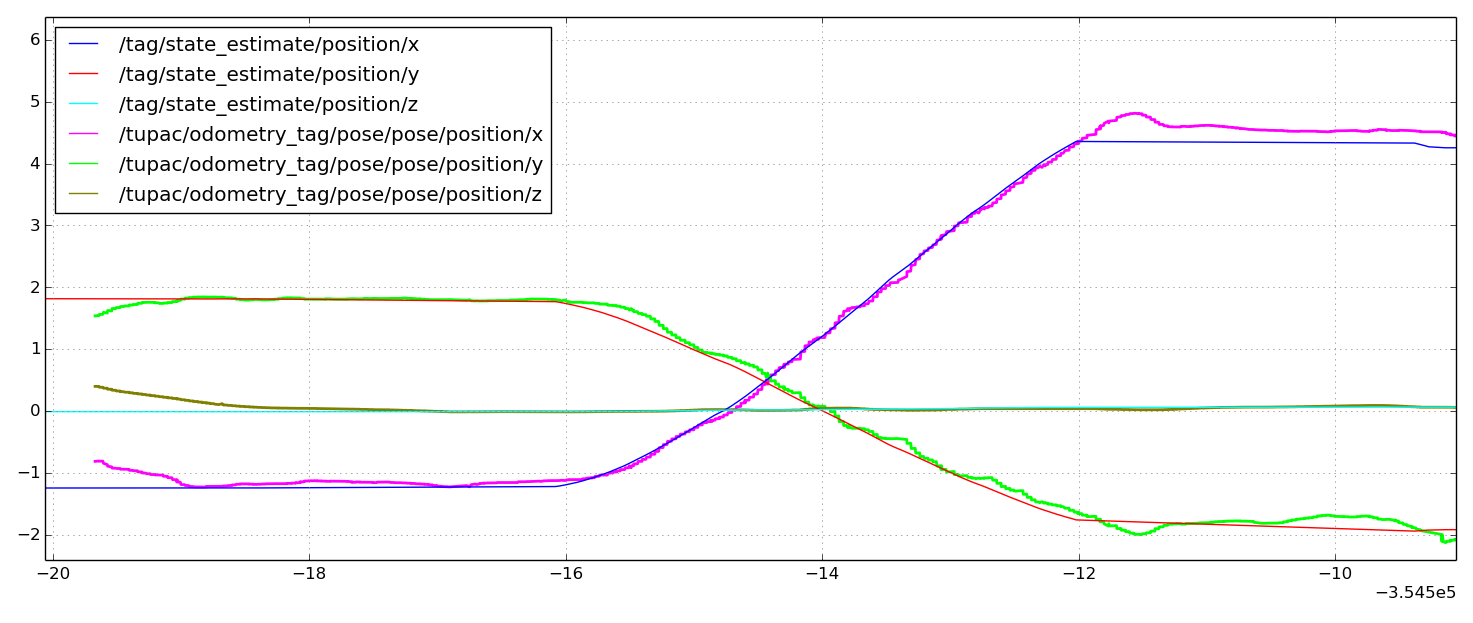
\includegraphics[width=0.97\textwidth]{img/position_real_world_fast.png}
      \caption{Real world test. Comparison between estimate position and ground truth for a platform moving at $2\frac{m}{s}$}
    \label{fig:ekf_position_real_fast}
\end{figure}

\section{State Prediction}
